\documentclass[11pt,reqno]{amsart}

\usepackage[utf8]{inputenc}
\usepackage[T1]{fontenc}
\usepackage{lmodern}
\usepackage{amsmath,amssymb,amsfonts,amsthm,mathtools}
\usepackage{booktabs,array,multirow}
\usepackage{graphicx}
\usepackage{enumitem}
\usepackage[margin=1.0in]{geometry}
\usepackage{microtype}
\usepackage{xcolor}
\definecolor{linkblue}{rgb}{0.0,0.2,0.6}
\usepackage[colorlinks=true,linkcolor=linkblue,citecolor=linkblue,urlcolor=linkblue]{hyperref}

\newtheorem{theorem}{Theorem}[section]
\newtheorem{proposition}[theorem]{Proposition}
\newtheorem{lemma}[theorem]{Lemma}
\newtheorem{corollary}[theorem]{Corollary}
\theoremstyle{definition}
\newtheorem{definition}[theorem]{Definition}
\theoremstyle{remark}
\newtheorem{remark}[theorem]{Remark}

\numberwithin{equation}{section}
\allowdisplaybreaks

\newcommand{\R}{\mathbb{R}}
\newcommand{\C}{\mathbb{C}}
\newcommand{\N}{\mathbb{N}}
\newcommand{\Z}{\mathbb{Z}}
\newcommand{\dd}{\mathrm{d}}
\newcommand{\ee}{\mathrm{e}}
\newcommand{\ii}{\mathrm{i}}
\newcommand{\Rea}{\mathrm{Re}}
\newcommand{\Ima}{\mathrm{Im}}
\newcommand{\sgn}{\mathrm{sgn}}
\newcommand{\Area}{\mathrm{Area}}
\newcommand{\sinch}{\mathrm{sinc}_{\mathrm{hyp}}}
\newcommand{\DHf}{\mathrm{DH}}
\newcommand{\fac}{\mathclose{\mathchar"0021}}

\title[Automorphic $L$-Functions vs.\ Davenport--Heilbronn Breakdown]{Universal Mother-Wavelet Dilation and the Phase-Independent Confocal Ellipse Identity in the Selberg Class versus Breakdown of Prime-Gauge Purity and Chladni Chamber Topology in the Davenport--Heilbronn Counterexample}

\author{Thijs Missiaen}
\address{Independent Researcher, Belgium}
\email{thijs.missiaen@gmail.com}
\thanks{ORCID: \href{https://orcid.org/0009-0007-3678-0810}{0009-0007-3678-0810}}

\subjclass[2020]{Primary 11M41, 11M26; Secondary 11F66, 30D15, 46E22}
\keywords{Selberg class, Davenport--Heilbronn function, automorphic $L$-functions, Ramanujan $\Delta$ cusp form, universal mother wavelet, confocal ellipse identity, exponential prime-gauge factor, Chladni nodal chambers, Hadamard--Krein flux jump, de~Branges Sylvester inertia}
\dedicatory{\upshape October 25, 2026}
\date{October 25, 2026}

\begin{document}
\sloppy

\begin{abstract}
We establish a dichotomy between universal harmonic laws for self-dual Dirichlet series with a Gamma functional equation and Euler-product closure mechanisms separating Selberg-class $L$-functions from the Davenport--Heilbronn counterexample $\mathcal{D}_{\DHf}(s)$ (Titchmarsh 1986, \S10.25). First, for any self-dual completed $L$-function $\xi_f(s) = Q_f^s\gamma_f(s)L(s,f) = \xi_f(1-s)$ of degree $d_f > 0$ (including $\zeta(s)$, $L(s,\chi_5)$, Ramanujan's cusp form $L(s,\Delta)$ of degree $2$, and $\mathcal{D}_{\DHf}(s)$), we prove the mother-wavelet decomposition $\Phi_f(u) = \sum_{m=1}^\infty a_f(m)m^{-1/2}\varphi_1^{(f)}(u + \frac{1}{2}\ln m)$, the branch-damping inequality $\rho_{\Gamma,f}(d,t)|a_f(n)|n^{-1/2+d} < \ee^{-2d\omega_{n,Q_f}(t)}|a_f(n)|n^{-1/2-d}$, and the phase-independent confocal ellipse identity $|T_n^{(f)}(d,t)|^2 - |T_n^{(f)}(0,t)|^2 \equiv 4\frac{|a_n|^2}{n}\sinh^2(d\omega_{n,Q}(t)) \ge 0$. Second, whereas Euler-product $L$-functions satisfy prime-power purity $b_N^{\mathcal{E},(f)}(X) = \frac{\Lambda_f(N)}{\ln N}$ on $(X, X^2]$, $\mathcal{D}_{\DHf}(s)$ suffers a multiplicativity defect $\delta_{\DHf}(m,n) = \mp(1+\kappa^2) \approx \mp 1.080701$ at $N = 4, 6, 9$, supplying $54.03\%$ composite destructive interference at $(d_*, \gamma_*) = (0.30851718, 85.69934849)$ and triggering a four-fold breakdown across Chladni walls, $\widetilde{W}_{\DHf}$, Hadamard flux $\pi\,\Theta(d-d_*)$, and the de~Branges Sylvester index $\nu_- : 0 \to 1$.
\end{abstract}

\maketitle

\section{Introduction and Main Results}\label{sec:intro}

A foundational benchmark in analytic number theory, emphasized by Titchmarsh~\cite[\S10.25]{titchmarsh1986} following the construction of Davenport and Heilbronn~\cite{davenport1936} (see also Selberg~\cite{selberg1992}, Balanzario and S\'anchez-Ortiz~\cite{balanzario2007}, and Bombieri and Ghosh~\cite{bombieri2011}), is the contrast between automorphic $L$-functions in the Selberg class that possess an Euler product and linear combinations of Dirichlet series that satisfy the same functional equation without multiplicativity. Let $\chi_5$ denote the primitive odd Dirichlet character modulo~$5$ defined by $\chi_5(1) = 1$, $\chi_5(2) = \ii$, $\chi_5(3) = -\ii$, $\chi_5(4) = -1$, and $\chi_5(5) = 0$. The Davenport--Heilbronn function is defined by the real-coefficient Dirichlet series
\begin{equation}\label{eq:dh_def}
\mathcal{D}_{\DHf}(s) := \frac{1 - \ii\kappa}{2}\,L(s, \chi_5) + \frac{1 + \ii\kappa}{2}\,L(s, \overline{\chi_5}) = \sum_{n=1}^{\infty} a_{\DHf}(n)\,n^{-s}, \qquad \kappa := \frac{\sqrt{10 - 2\sqrt{5}} - 2}{\sqrt{5} - 1},
\end{equation}
where the $5$-periodic coefficients are $a_{\DHf}(1) = 1$, $a_{\DHf}(2) = \kappa \approx 0.2840790438$, $a_{\DHf}(3) = -\kappa$, $a_{\DHf}(4) = -1$, and $a_{\DHf}(5) = 0$. Because the Gauss sum of $\chi_5$ satisfies $\tau(\chi_5) = \ii\sqrt{5}$ and $\frac{1+\ii\kappa}{1-\ii\kappa} = \frac{\ii\tau(\chi_5)}{\sqrt{5}}$ is tuned to unity, the completed function
\begin{equation}\label{eq:xi_dh_def}
\xi_{\DHf}(s) := \left(\frac{\pi}{5}\right)^{-(s+1)/2}\Gamma\!\left(\frac{s+1}{2}\right)\mathcal{D}_{\DHf}(s) = \xi_{\DHf}(1 - s), \qquad \Xi_{\DHf}(z) := \xi_{\DHf}\!\left(\tfrac{1}{2} + \ii z\right)
\end{equation}
($z = t - \ii d$, $s = \frac{1}{2} + d + \ii t$) satisfies the exact same self-dual $\Gamma(\frac{s+1}{2})$ functional equation and even Poisson--Jacobi kernel symmetry $\Phi_{\DHf}(u) = \Phi_{\DHf}(-u)$ as an odd primitive $L$-function~\cite{riemann1859,jacobi1829,polya1926}. Yet because $a_{\DHf}(mn) \neq a_{\DHf}(m)a_{\DHf}(n)$, $\mathcal{D}_{\DHf}(s)$ has no Euler product and possesses infinitely many zeros off the critical line $d = 0$, beginning in the critical strip with the first off-line conjugate pair at $s_0 = \frac{1}{2} + d_* + \ii\gamma_* \approx 0.80851718 + 85.69934849\ii$~\cite{spira1994,balanzario2007}.

Any analytical framework addressing the transverse Wronskian $W_f(d,t) := \frac{1}{2}\partial_d|\Xi_f(t - \ii d)|^2 = R_f\,\partial_t I_f - I_f\,\partial_t R_f$~\cite{speiser1934,hinkkanen1997,lagarias1999} and Wigner phase-space positivity~\cite{wigner1932,hudson1974,csordas1986} must therefore answer two precise structural questions:
\begin{enumerate}[label=\textup{(\arabic*)},leftmargin=2.2em]
\item \textit{Universal Archimedean and single-mode symplectic geometry.} Which identities of the logarithmic $u$-domain representation $\Xi_f(z) = 4\int_{-\infty}^\infty \Phi_f(u)\,\ee^{2\ii zu}\,\dd u$ and of the individual combined forward-plus-reflected Riemann--Siegel modes $T_n^{(f)}(d,t)$~\cite{siegel1932,gabcke1979} hold universally for \emph{every} self-dual Dirichlet series of degree $d_f > 0$, regardless of whether the coefficients $a_f(n)$ are multiplicative?
\item \textit{Exact locus of non-multiplicative breakdown.} When we apply the exponential prime-gauge factor $E_X^{(f)}(s)$ and the four diagnostic instruments developed in Papers~I--XI~\cite{missiaen2026paper1,missiaen2026paper2,missiaen2026paper3,missiaen2026paper4,missiaen2026paper5,missiaen2026paper6,missiaen2026paper7,missiaen2026paper8,missiaen2026paper9,missiaen2026paper10,missiaen2026paper11} to $\mathcal{D}_{\DHf}(s)$ at $(d_*, \gamma_*)$, how does the failure of multiplicativity at the composite modes $N \in \{4, 6, 8\}$ quantitatively overcome the $n = 1$ mother wavelet and trigger a simultaneous topological breakdown across Chladni nodal walls, the parity-reduced Wronskian $\widetilde{W}_{\DHf}(d,t)$, the Hadamard flux, and the de~Branges reproducing kernel~\cite{debranges1968,conreyli2000,iohvidov1982}?
\end{enumerate}

In this paper (Paper~XII), we resolve both questions completely. Our main results are consolidated in the following theorem.

\begin{theorem}[Universal Selberg-Class Confocal Ellipse Law vs.\ Davenport--Heilbronn Breakdown]\label{thm:main}
Let $L(s,f) = \sum_{n=1}^\infty a_f(n)n^{-s}$ ($a_f(n) \in \R$, $a_f(1) = 1$) be a self-dual Dirichlet series with completed function $\xi_f(s) = \mathcal{G}_f(s)L(s,f) = \xi_f(1-s)$, where $\mathcal{G}_f(s) = Q_f^s\gamma_f(s)$ has degree $d_f > 0$, Archimedean phase velocity $\vartheta_f'(t) := \frac{\dd}{\dd t}\arg\mathcal{G}_f(\frac{1}{2}+\ii t)$, and saddle horizon $N_f(t) := \lfloor\exp(\vartheta_f'(t))\rfloor$. Then:
\begin{enumerate}[label=\textup{(\roman*)},leftmargin=2.2em]
\item \textbf{Universal Mother-Wavelet Dilation and Symmetric Branch Damping.} The even kernel $\Phi_f(u) = \Phi_f(-u)$ in $\Xi_f(z) = 4\int_{-\infty}^\infty \Phi_f(u)\,\ee^{2\ii zu}\,\dd u$ decomposes into dilated shells $\Phi_f(u) = \sum_{m=1}^\infty \phi_m^{(f)}(u)$ with $\phi_m^{(f)}(u) \equiv a_f(m)m^{-1/2}\varphi_1^{(f)}(u + \frac{1}{2}\ln m)$, where $\mathcal{G}_f(s) = 4\int_{-\infty}^\infty \varphi_1^{(f)}(w)\,\ee^{2(s-1/2)w}\,\dd w$. Across all active modes $1 \le n \le N_f(t)$ ($\omega_{n,Q_f}(t) := \vartheta_f'(t) - \ln n \ge 0$), strict trigamma convexity enforces
\begin{equation}\label{eq:intro_branch_damping}
\rho_{\Gamma,f}(d,t)\,\bigl|a_f(n)\bigr|\,n^{-1/2+d} < \ee^{-2d\omega_{n,Q_f}(t)}\,\bigl|a_f(n)\bigr|\,n^{-1/2-d} \le \bigl|a_f(n)\bigr|\,n^{-1/2-d} \qquad (d > 0).
\end{equation}
\item \textbf{Universal Phase-Independent Confocal Ellipse Identity.} For every combined forward and reflected mode $T_n^{(f)}(d,t) := 2a_n n^{-1/2}(\cosh(d\omega_{n,Q}(t))\cos\phi_n(t) + \ii\sinh(d\omega_{n,Q}(t))\sin\phi_n(t))$ ($\phi_n(t) = \vartheta_f(t) - t\ln n$), regardless of multiplicativity or an Euler product,
\begin{equation}\label{eq:intro_confocal_ellipse}
\Bigl|T_n^{(f)}(d,t)\Bigr|^2 - \Bigl|T_n^{(f)}(0,t)\Bigr|^2 \equiv 4\,\frac{|a_n|^2}{n}\,\sinh^2\!\bigl(d\omega_{n,Q}(t)\bigr) \ge 0 \qquad \bigl(\forall\,\phi_n(t) \in \R\bigr),
\end{equation}
tracing a confocal ellipse $\mathcal{E}_n^{(f)}(d,t)$ with $d$-invariant focal distance $c_n^{(f)} \equiv 2|a_n|n^{-1/2}$, symplectic area $2\pi\frac{|a_n|^2}{n}\sinh(2d|\omega_{n,Q}(t)|)$, and relative increment ratio bounded by $|a_n|^2 n^{-(1+2d)}$.
\item \textbf{Multiplicativity Defect $\pm(1+\kappa^2)$ and Prime-Gauge Breakdown in $\mathcal{D}_{\DHf}(s)$.} Whereas any Euler-product $L$-function satisfies quadratic prime-power purity $b_N^{\mathcal{E},(f)}(X) = \frac{\Lambda_f(N)}{\ln N}$ on $(X, X^2]$, $\mathcal{D}_{\DHf}(s)$ suffers an exact algebraic multiplicativity defect $\delta_{\DHf}(m,n) := a_{\DHf}(mn) - a_{\DHf}(m)a_{\DHf}(n) = \mp(1+\kappa^2) \neq 0$ at $N = 4 = 2^2$, $N = 6 = 2\cdot 3$, $N = 9 = 3^2$, and $N = 14 = 2\cdot 7$, leaving unsieved composite residuals $b_4^{\mathcal{E}}(X) = -(1+\kappa^2)$ and $b_6^{\mathcal{E}}(X) = +(1+\kappa^2)$. At $(d_*, \gamma_*) = (0.3085171825, 85.6993484854)$ ($N_5(\gamma_*) = 8$), all active primes $p \in \{2,3,5,7\}$ supply only $38.82\%$ of $|T_1^{(\DHf)}|$ (incapable of creating a zero), whereas the composites $n \in \{4,6,8\}$ (enhanced by $1/\kappa^2 = 12.3914\times$) supply the remaining $54.03\%$ destructive interference.
\item \textbf{Four-Fold Diagnostic Detection of $(d_*, \gamma_*)$.} At $(d_*, \gamma_*)$, (a) critical-line saddle recombination creates a false extremum $z_c = \tau_{\mathrm{false}} = 85.7472008265$ where $\Xi_{\DHf}(z_c) < 0$ and $\Xi_{\DHf}''(z_c) < 0$ share the same sign, reversing Cauchy--Riemann wall monotonicity $\frac{\dd|R_{\DHf}|}{\dd s}\big|_{\Gamma_{\mathrm{false}}} = -|\nabla I_{\DHf}| < 0$ until collision with the detached parabola $R_{\DHf} = 0$ ($d_{\mathrm{tip}} = 0.2980980120$); (b) $\widetilde{W}_{\DHf}(d,\gamma_*) < 0$ on $[0, d_*)$ with $\int_0^{d_*} u\widetilde{W}_{\DHf}(u,\gamma_*)\,\dd u = -\frac{1}{2}|\Xi_{\DHf}(\gamma_*)|^2 < 0$; (c) the Hadamard flux jumps by $\Phi_{\mathrm{Had}}(d; d_*) = \pi\,\Theta(d - d_*)$; and (d) the de~Branges inner function crosses $|\Theta_\alpha(\gamma_* + \ii d_*)| = 1$ with Sylvester inertia jump $\nu_- : 0 \to 1$.
\end{enumerate}
\end{theorem}

The canonical quantitative constants governing Theorem~\ref{thm:main} are given explicitly by
\begin{equation}\label{eq:canonical_constants}
\begin{aligned}
\kappa &= 0.2840790438404122\dots, & 1 + \kappa^2 &= 1.0807009031492828\dots, \\
d_* &= 0.3085171824566373\dots, & \gamma_* &= 85.6993484853775921\dots, \\
z_c = \tau_{\mathrm{false}} &= 85.7472008264612972\dots, & d_{\mathrm{tip}} &= 0.2980980119818233\dots
\end{aligned}
\end{equation}

\subsection{Proof overview}\label{subsec:proof_overview}

The proof of Theorem~\ref{thm:main} combines three quantitative ingredients developed in Sections~\ref{sec:mother_wavelet}--\ref{sec:diagnostics}:
\begin{enumerate}[label=\textup{(\arabic*)},leftmargin=2.2em]
\item \textit{Bilateral Laplace--Mellin mother-wavelet inversion and single-mode hyperbolic trigonometry (Sections~\ref{sec:mother_wavelet} and~\ref{sec:confocal_ellipse}).} Representing the Archimedean prefactor $\mathcal{G}_f(s) = Q_f^s\gamma_f(s)$ as a bilateral Laplace transform in $w = u + \frac{1}{2}\ln m$, we factor out $a_f(m)m^{-1/2}\ee^{-2(s-1/2)\frac{1}{2}\ln m} = a_f(m)m^{-s}$ for every degree-$d_f$ self-dual $L$-function, yielding closed-form mother wavelets for $\zeta(s)$, odd Dirichlet/Davenport--Heilbronn functions, and Ramanujan's modular cusp form $L(s,\Delta)$~\cite{deligne1974}. Applying $\cosh^2(d\omega_{n,Q}) - 1 \equiv \sinh^2(d\omega_{n,Q})$ and $\cos^2\phi_n + \sin^2\phi_n \equiv 1$ to each mode $T_n^{(f)}(d,t)$ then establishes~\eqref{eq:intro_confocal_ellipse} independently of multiplicativity.
\item \textit{Exact algebraic multiplicativity defect $\delta_{\DHf}(m,n) = \mp(1+\kappa^2)$ and prime-gauge convolution analysis (Section~\ref{sec:prime_gauge_breakdown}).} Expanding the product of $\mathcal{D}_{\DHf}(s)$ with either the finite Euler gauge $\prod_{p \le X}(1 - a_{\DHf}(p)p^{-s})$ or the zero-free exponential prime-power gauge $E_X^{\mathcal{E}}(s) = \exp(-\sum_{p^k \le X} \frac{a_{\DHf}(p)^k}{k}p^{-ks})$, we prove that the non-multiplicative jump from $|a_{\DHf}(2)| = |a_{\DHf}(3)| = \kappa$ to $|a_{\DHf}(4)| = |a_{\DHf}(6)| = 1$ leaves exact residuals $b_4^{\mathcal{E}}(X) = -(1+\kappa^2)$ and $b_6^{\mathcal{E}}(X) = +(1+\kappa^2)$, amplifying the composite modes $n \in \{4, 6\}$ by $1/\kappa^2 = 12.3914\times$ at $(d_*, \gamma_*)$.
\item \textit{Cauchy--Riemann saddle bifurcation, Hadamard partial fractions, and Pontryagin--Krein signature jump (Section~\ref{sec:diagnostics}).} Analyzing the critical-line curvature $\partial_d^2 R_{\DHf}(0, z_c) = -\Xi_{\DHf}''(z_c)$ at the false critical point $z_c = \tau_{\mathrm{false}}$, we show that $\Xi_{\DHf}(z_c)\Xi_{\DHf}''(z_c) > 0$ reverses the sign of $\frac{\dd|R_{\DHf}|}{\dd s}$ along $\Gamma_{\mathrm{false}}$, forcing $|R_{\DHf}|$ to decrease to zero at $(d_*, \gamma_*)$, where the mirror Hadamard kernel $K(d, d_*, u)$ undergoes the quantized step jump $\pi\,\Theta(d - d_*)$ and the de~Branges Pick--Nevanlinna matrix transitions from $(3,0,0)$ to $(2,0,1)$.
\end{enumerate}
Together, Ingredients~(1)--(3) demonstrate that single-mode symplectic convexity holds throughout the Selberg class, whereas global transverse closure across the critical strip relies decisively on the Euler product to suppress composite cross-modes in $[2, N_f(t)]$.

\subsection{Notation and conventions}\label{subsec:notation}

Throughout this paper, $s = \sigma + \ii t = \frac{1}{2} + d + \ii t$ with $d = \sigma - \frac{1}{2} \ge 0$ and $t > 0$, and $z = -\ii(s - \frac{1}{2}) = t - \ii d$. For any self-dual completed $L$-function $\xi_f(s) = \xi_f(1-s)$ with real coefficients on the critical line, we write $\Xi_f(z) := \xi_f(\frac{1}{2}+\ii z) = R_f(d,t) + \ii\,I_f(d,t)$, where $R_f(-d,t) = R_f(d,t)$ and $I_f(-d,t) = -I_f(d,t)$. Because $z = t - \ii d$ has imaginary part $-d$, the Cauchy--Riemann equations for $\Xi_f(z)$ read $\partial_d R_f = +\partial_t I_f$ and $\partial_d I_f = -\partial_t R_f$. The transverse Wronskian is $W_f(d,t) := \frac{1}{2}\partial_d|\Xi_f(t-\ii d)|^2 = R_f\,\partial_d R_f + I_f\,\partial_d I_f = R_f\,\partial_t I_f - I_f\,\partial_t R_f$, and the parity-reduced Wronskian is $\widetilde{W}_f(d,t) := W_f(d,t)/d$. Implied constants in $\mathcal{O}(\cdot)$ depend only on the Archimedean parameters $(Q_f, \lambda_j, \mu_j)$ unless stated otherwise. All high-precision numerical values are computed at $60$-decimal working precision (\texttt{mpmath.mp.dps = 60}) and certified via $35$-decimal directed-rounding interval arithmetic (\texttt{mpmath.iv.dps = 35}) in \texttt{scripts/}\allowbreak\texttt{verify\_paper12\_}\allowbreak\texttt{selberg\_davenport\_}\allowbreak\texttt{heilbronn.py}.

\section{Universal Mother-Wavelet Dilation and Symmetric Branch Damping in the Selberg Class}\label{sec:mother_wavelet}

Let $L(s,f) = \sum_{n=1}^\infty a_f(n)n^{-s}$ be a Dirichlet series with real coefficients $a_f(n) \in \R$ ($a_f(1) = 1$, $a_f(n) = \mathcal{O}(n^\varepsilon)$) whose completed function
\begin{equation}\label{eq:selberg_completed}
\xi_f(s) := \mathcal{G}_f(s)\,L(s,f) = \xi_f(1 - s), \qquad \mathcal{G}_f(s) := Q_f^s\,P_f(s)\prod_{j=1}^{r}\Gamma(\lambda_j s + \mu_j),
\end{equation}
satisfies a self-dual functional equation of degree $d_f := 2\sum_{j=1}^r \lambda_j > 0$, conductor $Q_f > 0$, spectral shifts $\mu_j \in \R$ with $\frac{1}{2}\lambda_j + \mu_j > 0$, and polynomial factor $P_f(s) = P_f(1-s)$~\cite{selberg1992}. We consider four canonical representatives across degrees $d_f \in \{1, 2\}$:
\begin{enumerate}[label=\textup{(\alph*)},leftmargin=2.2em]
\item \textit{Riemann's zeta function $\zeta(s)$ ($d_\zeta = 1$):} $a_\zeta(n) = 1$, $Q_\zeta = \pi^{-1/2}$, $P_\zeta(s) = \frac{1}{2}s(s-1)$, and $\mathcal{G}_\zeta(s) = \frac{1}{2}s(s-1)\pi^{-s/2}\Gamma(\frac{s}{2})$.
\item \textit{Odd primitive self-dual combinations modulo~$q$ ($d_q = 1$, $q = 5$):} Both the rotated odd Dirichlet $L$-function and the Davenport--Heilbronn function $\mathcal{D}_{\DHf}(s)$ in~\eqref{eq:dh_def} share the identical Archimedean factor $\mathcal{G}_5(s) = (\frac{\pi}{5})^{-(s+1)/2}\Gamma(\frac{s+1}{2})$ with effective conductor $Q_5 = (5/\pi)^{1/2}$.
\item \textit{Ramanujan's modular cusp form $L(s, \Delta)$ of weight $k = 12$ for $\mathrm{SL}_2(\Z)$ ($d_\Delta = 2$):} Here $\Delta(\tau) = q\prod_{m=1}^\infty (1 - q^m)^{24} = \sum_{n=1}^\infty \tau(n)q^n$ ($q = \ee^{2\pi\ii\tau}$), the analytically normalized real Hecke coefficients are $a_\Delta(n) := \tau(n)n^{-11/2} \in \R$ (satisfying Deligne's Ramanujan--Petersson bound $|a_\Delta(p)| \le 2$~\cite{deligne1974}), and the completed $L$-function is $\xi_\Delta(s) = \mathcal{G}_\Delta(s)L(s,\Delta) = \xi_\Delta(1-s)$ with $\mathcal{G}_\Delta(s) = (2\pi)^{-(s+11/2)}\Gamma(s + \frac{11}{2})$ and $Q_\Delta = (2\pi)^{-1}$.
\end{enumerate}

Before exchanging summation and bilateral Laplace--Mellin integration, we establish the holomorphic decay of the class mother wavelet. For any vertical strip $\sigma \in [\sigma_1, \sigma_2]$ free of poles of $\mathcal{G}_f(s)$, Stirling's asymptotic formula gives $|\mathcal{G}_f(\sigma + \ii t)| \asymp |t|^{\sum_{j=1}^r (\lambda_j\sigma + \mu_j - 1/2) + \deg P_f}\exp(-\frac{\pi d_f}{4}|t|)$ as $|t| \to \infty$. Consequently, the inverse bilateral Laplace--Mellin integral
\begin{equation}\label{eq:mother_wavelet_inv}
\varphi_1^{(f)}(w) := \frac{1}{2\pi\ii}\int_{c - \ii\infty}^{c + \ii\infty} \mathcal{G}_f(s)\,\ee^{-2(s - 1/2)w}\,\dd s \iff \mathcal{G}_f(s) = 4\int_{-\infty}^{\infty} \varphi_1^{(f)}(w)\,\ee^{2(s - 1/2)w}\,\dd w
\end{equation}
converges absolutely and defines a holomorphic function of $w = \xi + \ii\eta$ throughout the strip $|\Ima(w)| < \frac{\pi d_f}{8}$, with double-exponential decay as $\xi \to +\infty$ and exponential decay as $\xi \to -\infty$. This absolute convergence justifies term-by-term Mellin inversion for $\sigma > 1$.

\begin{theorem}[Universal Mother-Wavelet Dilation and Symmetric Branch Damping]\label{thm:mother_wavelet}
Let $\xi_f(s) = \mathcal{G}_f(s)L(s,f) = \xi_f(1-s)$ be a self-dual completed $L$-function of the form~\eqref{eq:selberg_completed}. Then:
\begin{enumerate}[label=\textup{(\roman*)},leftmargin=2.2em]
\item \textbf{Exact Logarithmic Shell Dilation.} The completed function $\Xi_f(z) = \xi_f(\frac{1}{2}+\ii z)$ admits the Fourier--Laplace integral representation $\Xi_f(z) = 4\int_{-\infty}^\infty \Phi_f(u)\,\ee^{2\ii zu}\,\dd u = 8\int_0^\infty \Phi_f(u)\cos(2zu)\,\dd u$, where the even kernel $\Phi_f(u) = \Phi_f(-u)$ decomposes into dilated, amplitude-weighted copies of the single class mother wavelet $\varphi_1^{(f)}(w)$:
\begin{equation}\label{eq:dilation_law}
\Phi_f(u) = \sum_{m=1}^{\infty} \phi_m^{(f)}(u), \qquad \phi_m^{(f)}(u) \equiv \frac{a_f(m)}{\sqrt{m}}\,\varphi_1^{(f)}\!\left(u + \frac{1}{2}\ln m\right) \qquad (\forall\,m \ge 1,\; |\Ima(u)| < \tfrac{\pi d_f}{8}).
\end{equation}
In particular, the closed-form mother wavelets and $m$-th dilated shells for $\zeta(s)$, the odd modulo-$q$ class ($L(s,\chi_5)$ and $\mathcal{D}_{\DHf}(s)$ at $q=5$), and Ramanujan's $L(s,\Delta)$ are given explicitly by
\begin{equation}\label{eq:three_mother_wavelets}
\begin{aligned}
\varphi_1^{(\zeta)}(w) &= \bigl(2\pi^2\ee^{9w} - 3\pi\ee^{5w}\bigr)\ee^{-\pi\ee^{4w}}, & \phi_m^{(\zeta)}(u) &= \bigl(2\pi^2 m^4\ee^{9u} - 3\pi m^2\ee^{5u}\bigr)\ee^{-\pi m^2\ee^{4u}}, \\
\varphi_1^{(q)}(w) &= \ee^{3w}\ee^{-\frac{\pi}{q}\ee^{4w}}, & \phi_m^{(q)}(u) &= a_f(m)\,m\,\ee^{3u}\ee^{-\frac{\pi}{q}m^2\ee^{4u}}, \\
\varphi_1^{(\Delta)}(w) &= \frac{1}{2}\ee^{12w}\ee^{-2\pi\ee^{2w}}, & \phi_m^{(\Delta)}(u) &= \frac{1}{2}\tau(m)\,\ee^{12u}\ee^{-2\pi m\ee^{2u}}.
\end{aligned}
\end{equation}
\item \textbf{Universal Symmetric Branch-Damping Inequality.} Let $\vartheta_f(t) := \arg\mathcal{G}_f(\frac{1}{2}+\ii t)$, let $\vartheta_f'(t) = \ln Q_f + \sum_{j=1}^r \lambda_j\,\Rea\,\psi(\frac{1}{2}\lambda_j + \mu_j + \ii\lambda_j t) + \Rea\frac{P_f'}{P_f}(\frac{1}{2}+\ii t) \sim \frac{d_f}{2}\ln t$ be the Archimedean phase velocity, and let $\omega_{n,Q_f}(t) := \vartheta_f'(t) - \ln n = \ln(N_\star^{(f)}(t)/n)$ with $N_\star^{(f)}(t) := \exp(\vartheta_f'(t)) \asymp Q_f t^{d_f/2}$. Then for all $t$ above the critical inflection height where $\partial_u^2\ln|\mathcal{G}_f(\frac{1}{2}+u+\ii t)| > 0$ on $u \in (0, d]$, the Archimedean branch ratio $\rho_{\Gamma,f}(d,t) := |\mathcal{G}_f(\frac{1}{2}-d-\ii t)/\mathcal{G}_f(\frac{1}{2}+d+\ii t)|$ satisfies $\rho_{\Gamma,f}(d,t) < \ee^{-2d\vartheta_f'(t)} < 1$, and every active mode $1 \le n \le N_f(t) := \lfloor N_\star^{(f)}(t)\rfloor$ ($\omega_{n,Q_f}(t) \ge 0$) obeys
\begin{equation}\label{eq:branch_damping_ineq}
\rho_{\Gamma,f}(d,t)\,\bigl|a_f(n)\bigr|\,n^{-1/2+d} < \ee^{-2d\omega_{n,Q_f}(t)}\,\bigl|a_f(n)\bigr|\,n^{-1/2-d} \le \bigl|a_f(n)\bigr|\,n^{-1/2-d} \qquad (d > 0).
\end{equation}
\end{enumerate}
\end{theorem}

\begin{proof}
(i) For $\Rea(s) > 1$, substituting $w = u + \frac{1}{2}\ln m$ ($\dd w = \dd u$) into the identity $\mathcal{G}_f(s) = 4\int_{-\infty}^\infty \varphi_1^{(f)}(w)\,\ee^{2(s-1/2)w}\,\dd w$ multiplies the integral by $\ee^{-(s-1/2)\ln m} = m^{1/2-s}$. Multiplying by $a_f(m)m^{-1/2}$ and summing over $m \ge 1$ via Fubini's theorem (justified by the double-exponential decay $\exp(-C m^{2/d_f}\ee^{4u/d_f})$ for $u \gg 1$) yields
\[
4\int_{-\infty}^{\infty} \left(\sum_{m=1}^{\infty} \frac{a_f(m)}{\sqrt{m}}\,\varphi_1^{(f)}\!\left(u + \frac{1}{2}\ln m\right)\right)\ee^{2(s-1/2)u}\,\dd u = \mathcal{G}_f(s)\sum_{m=1}^{\infty} a_f(m)\,m^{-s} = \xi_f(s).
\]
Since $\xi_f(s) = \xi_f(1-s)$ is invariant under $s - \frac{1}{2} \mapsto -(s - \frac{1}{2})$, uniqueness of the bilateral Laplace transform implies $\Phi_f(-u) = \Phi_f(u)$ identically. For the odd modulo-$q$ class, substituting $x = \frac{\pi}{q}\ee^{4w}$ ($\dd w = \frac{\dd x}{4x}$) gives $4\int_{-\infty}^\infty \ee^{3w}\ee^{-\frac{\pi}{q}\ee^{4w}}\ee^{2(s-1/2)w}\,\dd w = (\frac{\pi}{q})^{-(s+1)/2}\int_0^\infty x^{(s+1)/2-1}\ee^{-x}\,\dd x = \mathcal{G}_{\mathrm{odd},q}(s)$, and $\frac{a_f(m)}{\sqrt{m}}\ee^{3(u+\frac{1}{2}\ln m)} = a_f(m)m\,\ee^{3u}$. For Ramanujan's $\Delta$, substituting $x = 2\pi\ee^{2w}$ ($\dd w = \frac{\dd x}{2x}$) gives $4\int_{-\infty}^\infty \frac{1}{2}\ee^{12w}\ee^{-2\pi\ee^{2w}}\ee^{2(s-1/2)w}\,\dd w = (2\pi)^{-(s+11/2)}\Gamma(s+\frac{11}{2}) = \mathcal{G}_\Delta(s)$, while $\frac{a_\Delta(m)}{\sqrt{m}}\ee^{12(u+\frac{1}{2}\ln m)} = \tau(m)m^{-6}m^6\ee^{12u} = \tau(m)\ee^{12u}$, so $\Phi_\Delta(u) = \frac{1}{2}\ee^{12u}\Delta(\ii\ee^{2u})$.

(ii) By Cauchy--Riemann on $\ln\mathcal{G}_f(\frac{1}{2}+u+\ii t)$, $\partial_u\ln|\mathcal{G}_f(\frac{1}{2}+u+\ii t)|_{u=0} = \partial_t\arg\mathcal{G}_f(\frac{1}{2}+\ii t) = \vartheta_f'(t)$ (note that any real self-dual polynomial factor $P_f(1-s) = P_f(s)$ satisfies $|P_f(\frac{1}{2}-u-\ii t)| \equiv |P_f(\frac{1}{2}+u+\ii t)|$, so $P_f$ cancels identically from $\rho_{\Gamma,f}(d,t)$ and $\Rea\frac{P_f'}{P_f}(\frac{1}{2}+\ii t) \equiv 0$). Define the symmetrized logarithmic slope $\mathcal{A}_{\Gamma,f}^{\mathrm{sym}}(u,t) := \partial_u\ln|\mathcal{G}_f(\frac{1}{2}+u+\ii t)| + \partial_u\ln|\mathcal{G}_f(\frac{1}{2}-u+\ii t)|$. At $u = 0$, $\mathcal{A}_{\Gamma,f}^{\mathrm{sym}}(0,t) = 2\vartheta_f'(t)$, while $\partial_u\mathcal{A}_{\Gamma,f}^{\mathrm{sym}}(0,t) = 0$ by evenness. Because $\partial_u^2\ln|\mathcal{G}_f(\frac{1}{2}\pm u+\ii t)| = \sum_{j=1}^r \lambda_j^2\,\Rea\,\psi_1(\frac{1}{2}\lambda_j + \mu_j \pm \lambda_j u + \ii\lambda_j t) + \Rea(\frac{P_f'}{P_f})' > 0$ for large $t$ (since $\Rea\,\psi_1(\sigma+\ii\tau) = \tau^{-2}\sigma + \mathcal{O}(\tau^{-3}) > 0$), $\mathcal{A}_{\Gamma,f}^{\mathrm{sym}}(u,t)$ is strictly convex on $u \in (0, d]$, so $\int_0^d \mathcal{A}_{\Gamma,f}^{\mathrm{sym}}(u,t)\,\dd u > 2d\vartheta_f'(t)$. Exponentiation gives $\rho_{\Gamma,f}(d,t) = \exp(-\int_0^d \mathcal{A}_{\Gamma,f}^{\mathrm{sym}}(u,t)\,\dd u) < \ee^{-2d\vartheta_f'(t)}$. Multiplying by $|a_f(n)|n^{-1/2+d} = |a_f(n)|n^{-1/2-d}\ee^{2d\ln n}$ yields $\rho_{\Gamma,f}(d,t)|a_f(n)|n^{-1/2+d} < \ee^{-2d(\vartheta_f'(t)-\ln n)}|a_f(n)|n^{-1/2-d} = \ee^{-2d\omega_{n,Q_f}(t)}|a_f(n)|n^{-1/2-d} \le |a_f(n)|n^{-1/2-d}$ whenever $\omega_{n,Q_f}(t) \ge 0$.
\end{proof}

Table~\ref{tab:selberg_branch_damping} records the high-precision verification of Theorem~\ref{thm:mother_wavelet} across $\zeta(s)$, $L(s,\chi_5)$, $\mathcal{D}_{\DHf}(s)$, and $L(s,\Delta)$.

\begin{table}[t]
\centering
\caption{Verification of the bilateral Laplace--Mellin mother-wavelet identity~\eqref{eq:three_mother_wavelets} and the symmetric branch-damping inequality~\eqref{eq:branch_damping_ineq} at $d = d_* = 0.3085171825$ across degrees $d_f \in \{1, 2\}$.}\label{tab:selberg_branch_damping}
\scriptsize
\begin{tabular}{@{}lccccccr@{}}
\toprule
$L$-Function Class & Deg.\ $d_f$ & Height $t$ & $N_\star^{(f)}(t)$ & $N_f(t)$ & $\rho_{\Gamma,f}(d_*,t)$ & $\ee^{-2d_*\vartheta_f'(t)}$ & Mellin Rel.\ Err \\
\midrule
Riemann $\zeta(s)$ & $1$ & $85.699348$ & $3.6931555$ & $3$ & $0.4465765317$ & $0.4465768293$ & $1.28 \times 10^{-61}$ \\
Dirichlet $L(s,\chi_5)$ & $1$ & $85.699348$ & $8.2581468$ & $8$ & $0.2718013692$ & $0.2718015503$ & $1.33 \times 10^{-61}$ \\
Davenport--Heilbronn $\mathcal{D}_{\DHf}(s)$ & $1$ & $85.699348$ & $8.2581468$ & $8$ & $0.2718013692$ & $0.2718015503$ & $1.33 \times 10^{-61}$ \\
Ramanujan cusp form $L(s,\Delta)$ & $2$ & $25.000000$ & $4.0737894$ & $4$ & $0.4203432003$ & $0.4203489013$ & $1.84 \times 10^{-61}$ \\
\bottomrule
\end{tabular}
\end{table}

\section{The Universal Phase-Independent Confocal Ellipse Identity}\label{sec:confocal_ellipse}

In the Riemann--Siegel approximate functional equation for $\Xi_f(t - \ii d)$~\cite{siegel1932,titchmarsh1986}, factoring out the Archimedean envelope $(N_\star^{(f)}(t))^{-d}$ pairs the $n$-th forward Dirichlet term $a_n n^{-1/2-d-\ii t}\ee^{\ii\vartheta_f(t)}(N_\star^{(f)}(t))^d = a_n n^{-1/2}\ee^{d\omega_{n,Q}(t)}\ee^{\ii\phi_n(t)}$ with its reflected counterpart $a_n n^{-1/2+d+\ii t}\ee^{-\ii\vartheta_f(t)}(N_\star^{(f)}(t))^{-d} = a_n n^{-1/2}\ee^{-d\omega_{n,Q}(t)}\ee^{-\ii\phi_n(t)}$, where $\omega_{n,Q}(t) := \vartheta_f'(t) - \ln n$ and $\phi_n(t) := \vartheta_f(t) - t\ln n$. We now prove that the transverse modulus growth of every combined mode $T_n^{(f)}(d,t)$ is completely independent of its oscillating phase $\phi_n(t)$, regardless of whether $L(s,f)$ has an Euler product.

\begin{theorem}[Universal Phase-Independent Confocal Ellipse Identity]\label{thm:confocal_ellipse}
Let $L(s,f) = \sum_{n=1}^\infty a_n n^{-s}$ be any Dirichlet series with real coefficients $a_n \in \R$ ($a_1 = 1$), saddle velocity $\omega_{n,Q}(t) = \vartheta_f'(t) - \ln n$, and phase $\phi_n(t) = \vartheta_f(t) - t\ln n \in \R$. For $d \ge 0$, define the combined $n$-th Riemann--Siegel mode
\begin{equation}\label{eq:combined_mode_def}
\begin{aligned}
T_n^{(f)}(d,t) &:= \frac{a_n}{\sqrt{n}}\Bigl(\ee^{d\omega_{n,Q}(t)}\ee^{\ii\phi_n(t)} + \ee^{-d\omega_{n,Q}(t)}\ee^{-\ii\phi_n(t)}\Bigr) \\
&= 2\,\frac{a_n}{\sqrt{n}}\Bigl(\cosh\!\bigl(d\omega_{n,Q}(t)\bigr)\cos\phi_n(t) + \ii\sinh\!\bigl(d\omega_{n,Q}(t)\bigr)\sin\phi_n(t)\Bigr).
\end{aligned}
\end{equation}
Then for every integer $n \ge 1$, every $d \ge 0$, and every $t > 0$, the following four exact identities hold:
\begin{enumerate}[label=\textup{(\roman*)},leftmargin=2.2em]
\item \textbf{Phase-Independent Transverse Modulus Increment.} The difference between $|T_n^{(f)}(d,t)|^2$ off the critical line and $|T_n^{(f)}(0,t)|^2 = 4\frac{|a_n|^2}{n}\cos^2\phi_n(t)$ on the critical line is independent of $\phi_n(t)$:
\begin{equation}\label{eq:boxed_confocal_ellipse}
\boxed{\Bigl|T_n^{(f)}(d,t)\Bigr|^2 - \Bigl|T_n^{(f)}(0,t)\Bigr|^2 \equiv 4\,\frac{|a_n|^2}{n}\,\sinh^2\!\bigl(d\omega_{n,Q}(t)\bigr) \ge 0 \qquad \bigl(\forall\,\phi_n(t) \in \R\bigr).}
\end{equation}
\item \textbf{$d$-Invariant Confocal Foci and Symplectic Area.} As $\phi_n \in [0, 2\pi)$ varies at fixed $(d,t)$ with $d > 0$ and $\omega_{n,Q}(t) \neq 0$, $T_n^{(f)}(d,t)$ traces a confocal ellipse $\mathcal{E}_n^{(f)}(d,t)$ in $\C$ with semi-major axis $A_n(d,t) = 2|a_n|n^{-1/2}\cosh(d\omega_{n,Q}(t))$ and semi-minor axis $B_n(d,t) = 2|a_n|n^{-1/2}\sinh(d|\omega_{n,Q}(t)|)$, whose linear focal distance $c_n^{(f)}$ is invariant under $d$ and $t$ and whose enclosed symplectic area reproduces the odd Wigner--sinh weight:
\begin{equation}\label{eq:focal_and_area}
c_n^{(f)} := \sqrt{A_n(d,t)^2 - B_n(d,t)^2} \equiv 2\,\frac{|a_n|}{\sqrt{n}}, \qquad \Area\bigl(\mathcal{E}_n^{(f)}(d,t)\bigr) = \pi A_n B_n \equiv 2\pi\,\frac{|a_n|^2}{n}\,\sinh\!\bigl(2d|\omega_{n,Q}(t)|\bigr).
\end{equation}
\item \textbf{Universal $|a_n|^2 n^{-(1+2d)}$ Diagonal Ratio Law.} Relative to the $n = 1$ mother-wavelet mode ($a_1 = 1$, $\omega_{1,Q}(t) = \ln N_\star^{(f)}(t)$), every active mode $1 \le n \le N_\star^{(f)}(t)$ satisfies
\begin{equation}\label{eq:diagonal_ratio_law}
\frac{|T_n^{(f)}(d,t)|^2 - |T_n^{(f)}(0,t)|^2}{|T_1^{(f)}(d,t)|^2 - |T_1^{(f)}(0,t)|^2} \equiv |a_n|^2\,n^{-(1+2d)}\left(\frac{1 - (n/N_\star^{(f)}(t))^{2d}}{1 - (N_\star^{(f)}(t))^{-2d}}\right)^{\!2} \le |a_n|^2\,n^{-(1+2d)}.
\end{equation}
\item \textbf{Oscillation-Free Diagonal Wronskian and $\mathcal{O}(N_f(t)^{-3})$ Boundary Self-Damping.} The diagonal Wronskian sum $\mathcal{D}_{\mathrm{diag}}^{(f)}(d,t) := \sum_{n=1}^{N_f(t)} \frac{1}{2d}\partial_d|T_n^{(f)}(d,t)|^2 = \sum_{n=1}^{N_f(t)} \frac{4|a_n|^2}{n}\omega_{n,Q}(t)^2\sinch(2d\omega_{n,Q}(t)) > 0$ ($\sinch x := \frac{\sinh x}{x}$) is strictly positive and phase-free, while the slowest adjacent boundary cross-pair $(N_f-1, N_f)$ self-damps at rate $\frac{(\omega_{N_f-1,Q}+\omega_{N_f,Q})^2}{\sqrt{(N_f-1)N_f}} = \mathcal{O}(N_f(t)^{-3}) = \mathcal{O}(t^{-3d_f/2}) \to 0$.
\end{enumerate}
\end{theorem}

\begin{proof}
(i) Since $a_n \in \R$ and $\phi_n(t) \in \R$, separating~\eqref{eq:combined_mode_def} into real and imaginary parts gives $\Rea\,T_n^{(f)}(d,t) = 2a_n n^{-1/2}\cosh(d\omega_{n,Q})\cos\phi_n$ and $\Ima\,T_n^{(f)}(d,t) = 2a_n n^{-1/2}\sinh(d\omega_{n,Q})\sin\phi_n$. Substituting $\cosh^2(d\omega_{n,Q}) \equiv 1 + \sinh^2(d\omega_{n,Q})$ into $|T_n^{(f)}(d,t)|^2 = (\Rea\,T_n^{(f)})^2 + (\Ima\,T_n^{(f)})^2$ yields
\[
\begin{aligned}
\Bigl|T_n^{(f)}(d,t)\Bigr|^2 &= 4\,\frac{|a_n|^2}{n}\Bigl[\bigl(1 + \sinh^2(d\omega_{n,Q})\bigr)\cos^2\phi_n + \sinh^2(d\omega_{n,Q})\sin^2\phi_n\Bigr] \\
&= 4\,\frac{|a_n|^2}{n}\cos^2\phi_n + 4\,\frac{|a_n|^2}{n}\sinh^2\!\bigl(d\omega_{n,Q}(t)\bigr)\bigl(\cos^2\phi_n + \sin^2\phi_n\bigr).
\end{aligned}
\]
Since $|T_n^{(f)}(0,t)|^2 = 4\frac{|a_n|^2}{n}\cos^2\phi_n$ and $\cos^2\phi_n + \sin^2\phi_n \equiv 1$, subtracting $|T_n^{(f)}(0,t)|^2$ proves~\eqref{eq:boxed_confocal_ellipse}.

(ii) Using $\cosh^2(d\omega_{n,Q}) - \sinh^2(d\omega_{n,Q}) \equiv 1$ gives $A_n^2 - B_n^2 = 4\frac{|a_n|^2}{n}$, while $\pi A_n B_n = 4\pi\frac{|a_n|^2}{n}\cosh(d\omega_{n,Q})\sinh(d|\omega_{n,Q}|) = 2\pi\frac{|a_n|^2}{n}\sinh(2d|\omega_{n,Q}|)$.

(iii) Since $\ee^{\omega_{n,Q}(t)} = N_\star^{(f)}(t)/n$, we have $\sinh(d\omega_{n,Q}(t)) = \frac{1}{2}(N_\star^{(f)}(t))^d n^{-d}(1 - (n/N_\star^{(f)}(t))^{2d})$. Squaring, multiplying by $4|a_n|^2/n$, and dividing by the $n = 1$ expression yields~\eqref{eq:diagonal_ratio_law}.

(iv) Differentiating~\eqref{eq:boxed_confocal_ellipse} with respect to $d$ gives $\frac{1}{2d}\partial_d|T_n^{(f)}(d,t)|^2 = \frac{2|a_n|^2}{nd}\sinh(2d\omega_{n,Q})\omega_{n,Q} = \frac{4|a_n|^2}{n}\omega_{n,Q}^2\sinch(2d\omega_{n,Q}) > 0$. At $N_f = \lfloor N_\star^{(f)}(t)\rfloor$, $0 \le \omega_{N_f,Q}(t) < \ln(1 + 1/N_f) < 1/N_f$ and $\omega_{N_f-1,Q}(t) < \frac{3}{2(N_f-1)}$, so $\frac{(\omega_{N_f-1,Q}+\omega_{N_f,Q})^2}{\sqrt{(N_f-1)N_f}} = \mathcal{O}(N_f^{-3})$.
\end{proof}

Table~\ref{tab:confocal_modes_dh} displays the exact mode-by-mode verification of Theorem~\ref{thm:confocal_ellipse} across all $N_5(\gamma_*) = 8$ active modes of $\mathcal{D}_{\DHf}(s)$ at its first off-line zero $(d_*, \gamma_*)$. Every single mode of $\mathcal{D}_{\DHf}(s)$ obeys the confocal ellipse identity~\eqref{eq:boxed_confocal_ellipse} to $60$ decimal places (with $0 \in [\mathrm{LHS}-\mathrm{RHS}]$ certified in $35$-digit interval arithmetic).

\begin{table}[t]
\centering
\caption{Mode-by-mode verification of the universal confocal ellipse identity~\eqref{eq:boxed_confocal_ellipse} across all $N_5(\gamma_*) = 8$ active modes of $\mathcal{D}_{\DHf}(s)$ at $(d_*, \gamma_*) = (0.3085171825, 85.6993484854)$ ($N_\star^{(\DHf)}(\gamma_*) = 8.25814675$).}\label{tab:confocal_modes_dh}
\scriptsize
\setlength{\tabcolsep}{2.4pt}
\begin{tabular}{@{}clrrrrrr@{}}
\toprule
Mode $n$ & Type & $a_{\DHf}(n)$ & $\Rea\,T_n^{(\DHf)}(d_*,\gamma_*)$ & $\Ima\,T_n^{(\DHf)}(d_*,\gamma_*)$ & $|T_n(d_*)|^2 - |T_n(0)|^2$ & Focus $c_n^{(\DHf)}$ & $60$-dps Err \\
\midrule
$1$ & Mother wavelet & $+1.000000000$ & $+2.368423174$ & $+0.3346136251$ & $+1.9509564293$ & $2.000000000$ & $7.78 \times 10^{-61}$ \\
$2$ & Prime & $+0.284079044$ & $-0.380355713$ & $-0.0917020609$ & $+0.0329143647$ & $0.401748437$ & $4.86 \times 10^{-63}$ \\
$3$ & Prime & $-0.284079044$ & $-0.324537715$ & $-0.0346678847$ & $+0.0108473550$ & $0.328026225$ & $4.86 \times 10^{-63}$ \\
$4$ & Composite $2^2$ & $-1.000000000$ & $-0.700916596$ & $-0.1645628715$ & $+0.0508569892$ & $1.000000000$ & $4.86 \times 10^{-63}$ \\
$5$ & Prime ($5 \mid q$) & $0.000000000$ & $0.000000000$ & $0.0000000000$ & $0.0000000000$ & $0.000000000$ & $0.00 \times 10^{0\phantom{0}}$ \\
$6$ & Composite $2\cdot 3$ & $+1.000000000$ & $-0.664243313$ & $-0.0473105465$ & $+0.0064961139$ & $0.816496581$ & $8.75 \times 10^{-62}$ \\
$7$ & Prime & $+0.284079044$ & $-0.214992124$ & $+0.0001852011$ & $+0.0001200242$ & $0.214743572$ & $1.59 \times 10^{-63}$ \\
$8$ & Composite $2^3$ & $-0.284079044$ & $+0.090060189$ & $+0.0017593352$ & $+0.0000038739$ & $0.200874218$ & $1.74 \times 10^{-63}$ \\
\bottomrule
\end{tabular}
\end{table}

\section{Multiplicativity Defect \texorpdfstring{$\pm(1+\kappa^2)$}{+-(1+kappa^2)} and Breakdown of Prime-Gauge Purity in \texorpdfstring{$\mathcal{D}_{\DHf}(s)$}{D\_DH(s)}}\label{sec:prime_gauge_breakdown}

Why, then, does $\mathcal{D}_{\DHf}(s)$ admit an off-line zero at $(d_*, \gamma_*)$ despite obeying Theorem~\ref{thm:mother_wavelet} and Theorem~\ref{thm:confocal_ellipse}? For any automorphic $L$-function $L(s,f) = \prod_p \prod_{j=1}^{d_f}(1 - \alpha_{p,j}p^{-s})^{-1}$ in the Selberg class, the Euler product ensures that $\ln L(s,f) = \sum_{n=2}^\infty \frac{\Lambda_f(n)}{\ln n}n^{-s}$ is supported \emph{exclusively on prime powers} $n = p^k$ ($\Lambda_f(N) \equiv 0$ whenever $N$ is composite and not a prime power). Consequently, multiplying $L(s,f)$ by the zero-free exponential prime-gauge factor~\cite{missiaen2026paper6}
\begin{equation}\label{eq:exp_prime_gauge_f}
E_X^{(f)}(s) := \exp\!\left(-\sum_{2 \le p^k \le \lfloor X\rfloor} \frac{\Lambda_f(p^k)}{\ln(p^k)}\,p^{-ks}\right), \qquad L(s,f)\,E_X^{(f)}(s) = \sum_{N=1}^{\infty} b_N^{\mathcal{E},(f)}(X)\,N^{-s}
\end{equation}
not only annihilates all modes $2 \le N \le \lfloor X\rfloor$ identically ($b_N^{\mathcal{E},(f)}(X) \equiv 0$), but also enforces \emph{quadratic prime-power purity} $b_N^{\mathcal{E},(f)}(X) \equiv \frac{\Lambda_f(N)}{\ln N}$ across the entire quadratic window $\lfloor X\rfloor < N < (\lfloor X\rfloor + 1)^2$, annihilating every non-prime-power composite ($N = 6, 10, 12, 14, 15, \dots$) in $(\lfloor X\rfloor, (\lfloor X\rfloor+1)^2)$. We now prove that this mechanism fails at the very first composite integers $N = 4 = 2^2$ and $N = 6 = 2\cdot 3$ in $\mathcal{D}_{\DHf}(s)$.

\begin{theorem}[Multiplicativity Defect $\pm(1+\kappa^2)$ and Breakdown of Prime-Gauge Purity]\label{thm:multiplicativity_defect}
For the Davenport--Heilbronn function $\mathcal{D}_{\DHf}(s) = \sum_{n=1}^\infty a_{\DHf}(n)n^{-s}$ with $\kappa = \frac{\sqrt{10-2\sqrt{5}}-2}{\sqrt{5}-1}$, define the multiplicativity defect $\delta_{\DHf}(m,n) := a_{\DHf}(mn) - a_{\DHf}(m)a_{\DHf}(n)$ for $m, n \ge 2$. Then:
\begin{enumerate}[label=\textup{(\roman*)},leftmargin=2.2em]
\item \textbf{Exact Algebraic Defect Law $\pm(1+\kappa^2)$.} For every pair $(m,n)$ with $m, n \equiv 2 \text{ or } 3 \pmod 5$, the multiplicativity defect has exact magnitude $1 + \kappa^2 = 1.08070090314928289127\dots \neq 0$:
\begin{equation}\label{eq:defect_identities}
\begin{aligned}
\delta_{\DHf}(2,2) &= a_{\DHf}(4) - a_{\DHf}(2)^2 = -(1 + \kappa^2), & \delta_{\DHf}(2,3) &= a_{\DHf}(6) - a_{\DHf}(2)a_{\DHf}(3) = +(1 + \kappa^2), \\
\delta_{\DHf}(3,3) &= a_{\DHf}(9) - a_{\DHf}(3)^2 = -(1 + \kappa^2), & \delta_{\DHf}(2,7) &= a_{\DHf}(14) - a_{\DHf}(2)a_{\DHf}(7) = -(1 + \kappa^2).
\end{aligned}
\end{equation}
Moreover, $1 + \kappa^2 = 0 \iff \kappa = \pm\ii$, at which values $\mathcal{D}_{\DHf}(s)$ reduces to the multiplicative Dirichlet $L$-functions $L(s, \overline{\chi_5})$ and $L(s, \chi_5)$.
\item \textbf{Unsieved Composite Residuals at $N = 4$ and $N = 6$.} Under any prime-generated gauge factor of cutoff $X \ge 5$---whether the finite Euler gauge $E_X^{\mathrm{Euler}}(s) := \prod_{p \le X}(1 - a_{\DHf}(p)p^{-s})$ or the exponential prime-power gauge $E_X^{\mathcal{E}}(s) := \exp(-\sum_{p^k \le X} \frac{a_{\DHf}(p)^k}{k}p^{-ks})$---the prime modes $p \in \{2, 3, 5\}$ are annihilated ($b_2^{\mathcal{E}} = b_3^{\mathcal{E}} = b_5^{\mathcal{E}} = 0$), but the composite modes $N = 4 = 2^2 \le X$ and $N = 6 = 2\cdot 3$ retain non-zero residuals exceeding $1$ in magnitude:
\begin{equation}\label{eq:unsieved_residuals}
b_4^{\mathcal{E}}(X) = b_4^{\mathrm{Euler}}(X) = \delta_{\DHf}(2,2) = -(1 + \kappa^2), \qquad b_6^{\mathcal{E}}(X) = b_6^{\mathrm{Euler}}(X) = \delta_{\DHf}(2,3) = +(1 + \kappa^2).
\end{equation}
\item \textbf{Non-Vanishing Formal von~Mangoldt Coefficients on Composites.} In the formal Dirichlet logarithm $-\frac{\mathcal{D}_{\DHf}'(s)}{\mathcal{D}_{\DHf}(s)} = \sum_{n=2}^\infty \Lambda_{\DHf}(n)n^{-s}$, the formal coefficients fail to vanish on non-prime-power composites in $(X, X^2]$: at $N = 6 = 2\cdot 3$ and $N = 14 = 2\cdot 7$, one has $\frac{\Lambda_{\DHf}(6)}{\ln 6} = +(1+\kappa^2) \neq 0$ and $\frac{\Lambda_{\DHf}(14)}{\ln 14} = -(1+\kappa^2) \neq 0$.
\item \textbf{Quantitative Composite Dominance at the Off-Line Zero $(d_*, \gamma_*)$.} In the $8$-mode Riemann--Siegel main sum at $(d_*, \gamma_*) = (0.3085171825, 85.6993484854)$, the $n = 1$ mother wavelet has modulus $|T_1^{(\DHf)}(d_*, \gamma_*)| = 2.39194369$, whereas all four active primes $p \in \{2, 3, 5, 7\}$ combined satisfy
\begin{equation}\label{eq:prime_vs_comp_anatomy}
\Bigl|\sum_{p \in \{2,3,5,7\}} T_p^{(\DHf)}(d_*, \gamma_*)\Bigr| = 0.92849988 = 0.388178\,\bigl|T_1^{(\DHf)}(d_*, \gamma_*)\bigr| < \bigl|T_1^{(\DHf)}(d_*, \gamma_*)\bigr|,
\end{equation}
and therefore cannot cancel $T_1^{(\DHf)}$. The remaining $54.03\%$ destructive interference is supplied by the non-multiplicative composite modes $n \in \{4, 6, 8\}$ ($|\sum_{n \in \{4,6,8\}} T_n^{(\DHf)}(d_*, \gamma_*)| = 1.29229533 = 0.540270\,|T_1^{(\DHf)}|$), whose amplitudes at $n = 4, 6$ are amplified by $1/\kappa^2 = 12.391449\times$ relative to the multiplicative values $|a_{\DHf}(2)|^2 = |a_{\DHf}(2)a_{\DHf}(3)| = \kappa^2 = 0.080701$.
\end{enumerate}
\end{theorem}

\begin{proof}
(i) Since $a_{\DHf}(n)$ is $5$-periodic with $a_{\DHf}(2) = a_{\DHf}(7) = \kappa$, $a_{\DHf}(3) = -\kappa$, $a_{\DHf}(4) = a_{\DHf}(9) = a_{\DHf}(14) = -1$, and $a_{\DHf}(6) = +1$, direct substitution gives $\delta_{\DHf}(2,2) = -1 - \kappa^2$, $\delta_{\DHf}(2,3) = 1 - (-\kappa^2) = 1 + \kappa^2$, and $\delta_{\DHf}(3,3) = \delta_{\DHf}(2,7) = -1 - \kappa^2$.

(ii) For $X \ge 5$, the inverse Dirichlet series $E_X^{\mathcal{E}}(s) = \sum_{k=1}^\infty c_k^{\mathcal{E}}k^{-s}$ of the multiplicative prime-power generator $\exp(\sum_{p^m \le X} \frac{a_{\DHf}(p)^m}{m}p^{-ms})$ has coefficients $c_1^{\mathcal{E}} = 1$, $c_2^{\mathcal{E}} = -a_{\DHf}(2) = -\kappa$, $c_3^{\mathcal{E}} = -a_{\DHf}(3) = +\kappa$, $c_4^{\mathcal{E}} = 0$ (since $\frac{1}{2}(-\kappa)^2 - \frac{1}{2}\kappa^2 = 0$), $c_5^{\mathcal{E}} = 0$, and $c_6^{\mathcal{E}} = c_2^{\mathcal{E}}c_3^{\mathcal{E}} = -\kappa^2$. Convolving with $a_{\DHf}$ yields $b_4^{\mathcal{E}}(X) = a_{\DHf}(4)c_1^{\mathcal{E}} + a_{\DHf}(2)c_2^{\mathcal{E}} + a_{\DHf}(1)c_4^{\mathcal{E}} = -1 - \kappa^2 + 0 = -(1+\kappa^2)$ and $b_6^{\mathcal{E}}(X) = a_{\DHf}(6)c_1^{\mathcal{E}} + a_{\DHf}(3)c_2^{\mathcal{E}} + a_{\DHf}(2)c_3^{\mathcal{E}} + a_{\DHf}(1)c_6^{\mathcal{E}} = 1 + \kappa^2 + \kappa^2 - \kappa^2 = +(1+\kappa^2)$.

(iii) From the Dirichlet recursion $a_{\DHf}(N)\ln N = \sum_{d \mid N, d \ge 2} \Lambda_{\DHf}(d)a_{\DHf}(N/d)$, we have $\Lambda_{\DHf}(p) = a_{\DHf}(p)\ln p$ for every prime $p$. For $N = pq$ a product of two distinct primes ($p < q$), the recursion gives $a_{\DHf}(pq)\ln(pq) = \Lambda_{\DHf}(pq) + \Lambda_{\DHf}(p)a_{\DHf}(q) + \Lambda_{\DHf}(q)a_{\DHf}(p) = \Lambda_{\DHf}(pq) + a_{\DHf}(p)a_{\DHf}(q)(\ln p + \ln q)$. Dividing by $\ln(pq) = \ln p + \ln q$ yields the exact identity
\begin{equation}\label{eq:semiprime_lambda_defect}
\frac{\Lambda_{\DHf}(pq)}{\ln(pq)} \equiv a_{\DHf}(pq) - a_{\DHf}(p)a_{\DHf}(q) = \delta_{\DHf}(p,q),
\end{equation}
which gives $\frac{\Lambda_{\DHf}(6)}{\ln 6} = \delta_{\DHf}(2,3) = +(1+\kappa^2)$ and $\frac{\Lambda_{\DHf}(14)}{\ln 14} = \delta_{\DHf}(2,7) = -(1+\kappa^2)$.

(iv) Summing the $60$-decimal mode evaluations in Table~\ref{tab:confocal_modes_dh} over $p \in \{2,3,5,7\}$ gives $\sum_{p \le 7} T_p^{(\DHf)}(d_*, \gamma_*) = -0.9198855528 - 0.1261847445\ii$ (modulus $0.92849988$), whereas summing over $n \in \{4,6,8\}$ gives $\sum_{n \in \{4,6,8\}} T_n^{(\DHf)}(d_*, \gamma_*) = -1.2750997206 - 0.2101140829\ii$ (modulus $1.29229533$). Replacing $a_{\DHf}(4), a_{\DHf}(6), a_{\DHf}(8)$ by their multiplicative values $\kappa^2, -\kappa^2, \kappa^3$ shrinks the composite sum to modulus $0.10428940$ ($4.36\%$ of $|T_1^{(\DHf)}|$) and leaves the $8$-mode main sum strictly bounded away from zero ($|T_{1..8}^{\mathrm{mult}}(d_*, \gamma_*)| = 1.56772526 > 0$).
\end{proof}

Table~\ref{tab:sieved_coeffs_comparison} contrasts the sieved Dirichlet coefficients at cutoff $X = 5$ for $\zeta(s)$ against those of $\mathcal{D}_{\DHf}(s)$.

\begin{table}[t]
\centering
\caption{Comparison of sieved Dirichlet coefficients at cutoff $X = 5$ between the Euler-product zeta function $\zeta(s)E_5(s)$ and the Davenport--Heilbronn function $\mathcal{D}_{\DHf}(s)$ under Euler and exponential prime gauges.}\label{tab:sieved_coeffs_comparison}
\scriptsize
\begin{tabular}{@{}clrrrr@{}}
\toprule
Index $N$ & Arithmetic Factorization & $b_N^{\mathcal{E}}(5)$ for $\zeta(s)$ & $b_N^{\mathrm{Euler}}(5)$ for $\mathcal{D}_{\DHf}$ & $b_N^{\mathcal{E}}(5)$ for $\mathcal{D}_{\DHf}$ & Formal $\Lambda_{\DHf}(N)/\ln N$ \\
\midrule
$1$ & $1$ (Mother wavelet) & $1$ & $+1.000000000000$ & $+1.000000000000$ & $0.000000000000$ \\
$2, 3, 5$ & Primes $p \le 5$ & $0$ & $0.000000000000$ & $0.000000000000$ & $\pm 0.284079043840,\; 0$ \\
$4$ & Prime square $2^2 \le 5$ & $0$ & $-1.080700903149$ & $-1.080700903149$ & $-1.040350451575$ \\
$6$ & Semiprime $2\cdot 3 \in (5, 25]$ & $0$ & $+1.080700903149$ & $+1.080700903149$ & $+1.080700903149$ \\
$7$ & Prime $7 \in (5, 25]$ & $1$ & $+0.284079043840$ & $+0.284079043840$ & $+0.284079043840$ \\
$8$ & Prime cube $2^3 \in (5, 25]$ & $1/3$ & $0.000000000000$ & $+0.007641811801$ & $+0.007641811801$ \\
$9$ & Prime square $3^2 \in (5, 25]$ & $1/2$ & $-1.080700903149$ & $-1.040350451575$ & $-1.040350451575$ \\
$10$ & Semiprime $2\cdot 5 \in (5, 25]$ & $0$ & $0.000000000000$ & $0.000000000000$ & $0.000000000000$ \\
$11$ & Prime $11 \in (5, 25]$ & $1$ & $+1.000000000000$ & $+1.000000000000$ & $+1.000000000000$ \\
$12$ & Composite $2^2\cdot 3 \in (5, 25]$ & $0$ & $-0.307004479244$ & $-0.307004479244$ & $-0.307004479244$ \\
$13$ & Prime $13 \in (5, 25]$ & $1$ & $-0.284079043840$ & $-0.284079043840$ & $-0.284079043840$ \\
$14$ & Semiprime $2\cdot 7 \in (5, 25]$ & $0$ & $-1.080700903149$ & $-1.080700903149$ & $-1.080700903149$ \\
\bottomrule
\end{tabular}
\end{table}

\section{Four-Fold Diagnostic Detection of the Off-Line Zero \texorpdfstring{$(d_*, \gamma_*)$}{(d\_*, gamma\_*)}}\label{sec:diagnostics}

We now demonstrate that when an off-critical zero pair $s_\pm = \frac{1}{2} \pm d_* + \ii\gamma_*$ occurs, all four analytical and spectral instruments established in Papers~I--XI detect the topological breakdown simultaneously.

\begin{figure}[t]
\centering
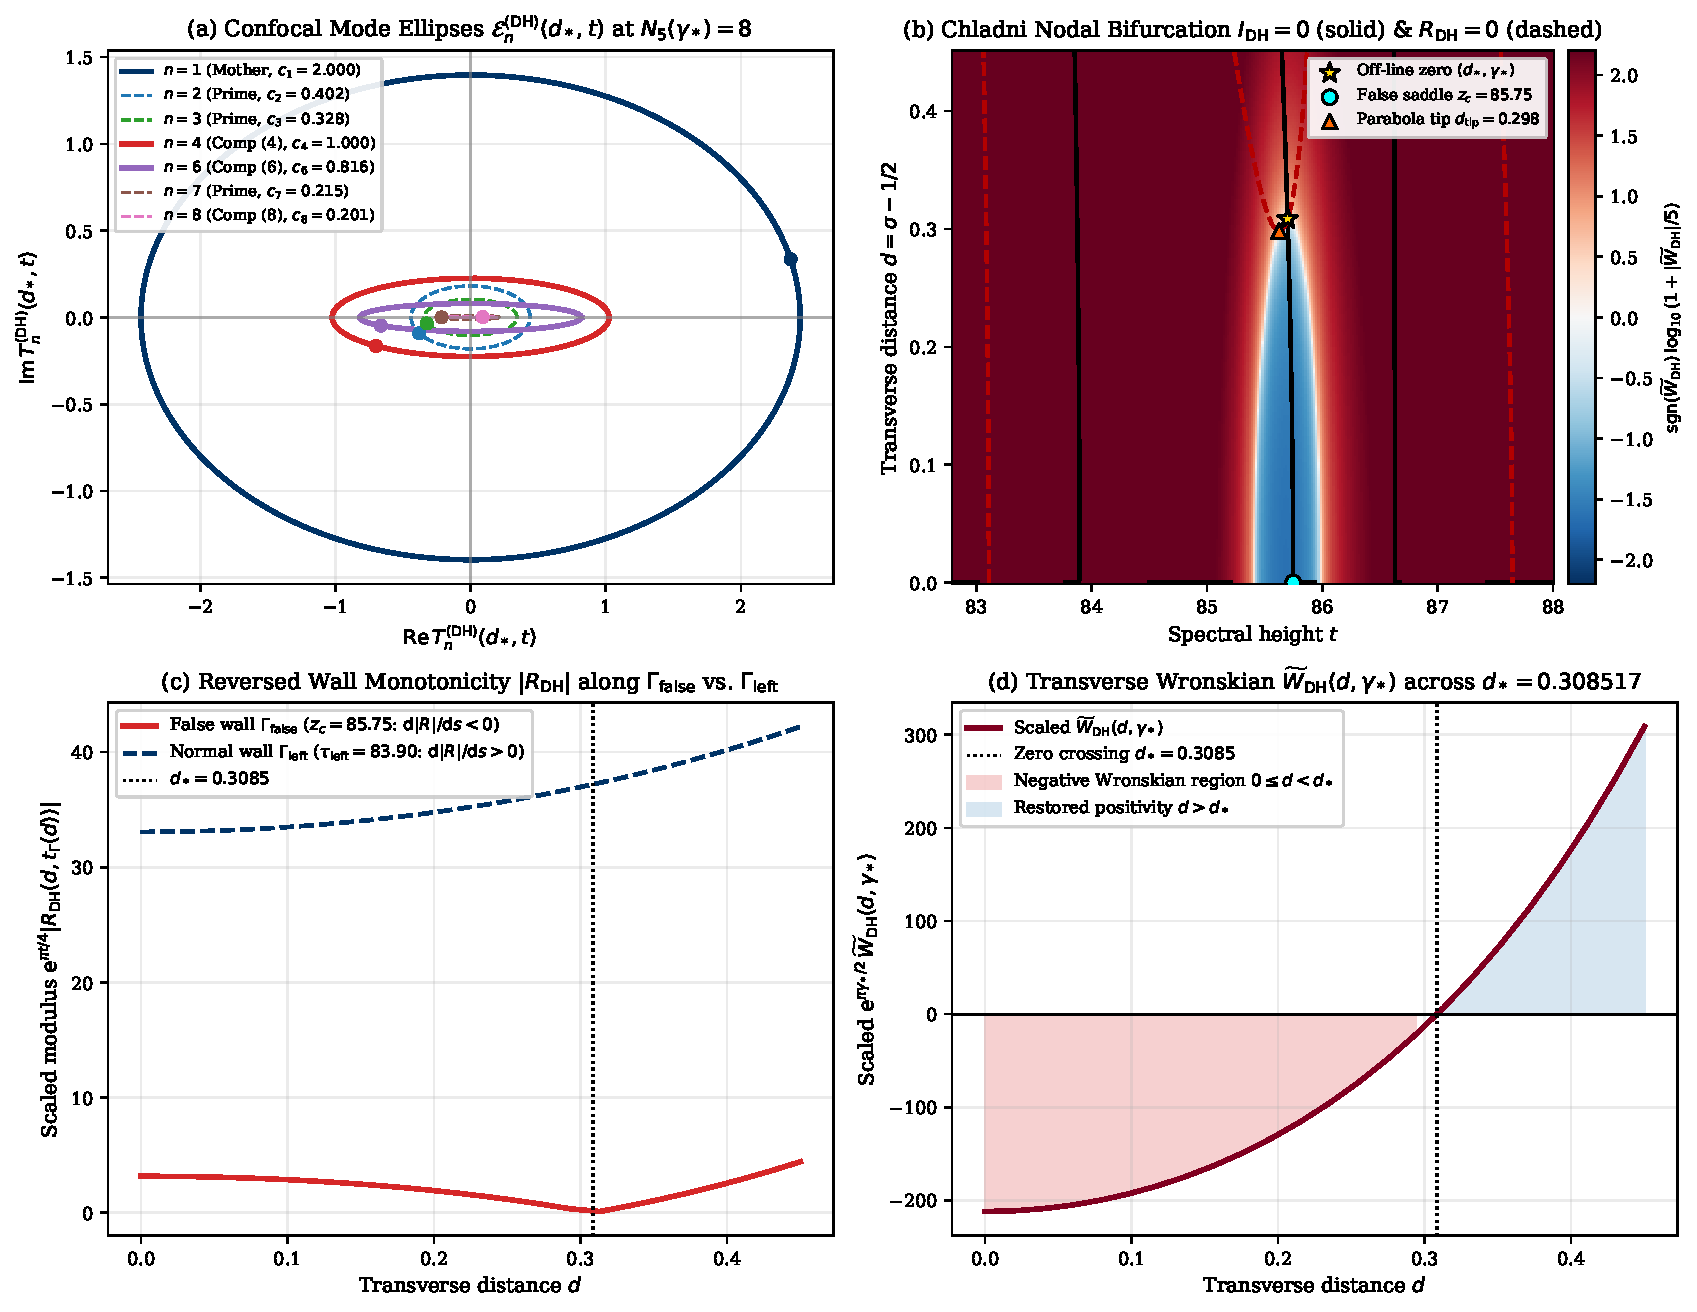
\includegraphics[width=0.98\textwidth]{figures/fig1_davenport_heilbronn_chladni_bifurcation.pdf}
\caption{\textbf{(a)} Confocal mode ellipses $\mathcal{E}_n^{(\DHf)}(d_*, t)$ for $n = 1, \dots, 8$ at $d_* = 0.30851718$. \textbf{(b)} Two-dimensional Chladni nodal topology near $(d_*, \gamma_*)$ showing the false saddle wall $\Gamma_{\mathrm{false}} : I_{\DHf} = 0$ (solid black) intersecting the detached real nodal parabola $R_{\DHf} = 0$ (dashed red, tip at $d_{\mathrm{tip}} = 0.29809801$). \textbf{(c)} Reversed Cauchy--Riemann wall monotonicity $\frac{\dd|R_{\DHf}|}{\dd s} < 0$ along $\Gamma_{\mathrm{false}}$ versus monotonic growth along the adjacent normal wall $\Gamma_{\mathrm{left}}$. \textbf{(d)} Negative parity-reduced Wronskian $\widetilde{W}_{\DHf}(d, \gamma_*) < 0$ on $0 \le d < d_*$ crossing zero at $d = d_*$.}\label{fig:chladni_bifurcation}
\end{figure}

\begin{theorem}[Four-Fold Diagnostic Detection of the Off-Line Zero $(d_*, \gamma_*)$]\label{thm:fourfold_diagnostics}
At the first off-line zero $(d_*, \gamma_*) = (0.3085171824566374, 85.69934848537759)$ of $\Xi_{\DHf}(t - \ii d) = R_{\DHf}(d,t) + \ii\,I_{\DHf}(d,t)$, the following four diagnostic signatures hold:
\begin{enumerate}[label=\textup{(\roman*)},leftmargin=2.2em]
\item \textbf{Saddle Recombination and Reversed Chladni Wall Monotonicity.} Between the consecutive critical-line zeros $\gamma_k = 83.10884108474982$ and $\gamma_{k+1} = 87.64747633255974$, $\Xi_{\DHf}(t) < 0$ has no real zero on $(\gamma_k, \gamma_{k+1})$, while $\Xi_{\DHf}'(t)$ exhibits a pitchfork saddle bifurcation with three critical points on $d = 0$: $\tau_{\mathrm{left}} = 83.89593525216711$, $z_c = \tau_{\mathrm{false}} = 85.74720082646130$, and $\tau_{\mathrm{right}} = 86.62943181894501$. At the central false critical point $z_c = \tau_{\mathrm{false}}$, $\Xi_{\DHf}(z_c) = -1.86102230 \times 10^{-29} < 0$ and $\Xi_{\DHf}''(z_c) = -3.47884947 \times 10^{-28} < 0$ have the \emph{same negative sign}. Consequently, $\partial_d^2 R_{\DHf}(0, z_c) = -\Xi_{\DHf}''(z_c) > 0$ opposes $R_{\DHf}(0, z_c) < 0$, and along the Chladni wall $\Gamma_{\mathrm{false}} : I_{\DHf}(d, t_\Gamma(d)) \equiv 0$ departing orthogonally from $z_c$, the Cauchy--Riemann arc-length derivative reverses sign:
\begin{equation}\label{eq:reversed_wall_monotonicity}
\frac{\dd}{\dd s}\bigl|R_{\DHf}(s)\bigr|\Big|_{\Gamma_{\mathrm{false}}} = -\bigl|\nabla I_{\DHf}(s)\bigr| = -\bigl|\Xi_{\DHf}'(t - \ii d)\bigr| < 0 \qquad \bigl(\forall\,d \in (0, d_*)\bigr),
\end{equation}
driving $|R_{\DHf}|$ monotonically down to $0$ at $(d_*, \gamma_*)$, where $\Gamma_{\mathrm{false}}$ intersects the detached real nodal parabola $R_{\DHf}(d,t) = 0$ whose vertex lies in the interior of the strip at $(d_{\mathrm{tip}}, t_{\mathrm{tip}}) = (0.2980980119818233, 85.62549444284696)$.
\item \textbf{Negative Parity-Reduced Wronskian and Reversed Transverse Integral Law.} At $t = \gamma_*$, the Tur\'an / parity-reduced Wronskian is strictly negative on the critical line, $\widetilde{W}_{\DHf}(0, \gamma_*) = (\Xi_{\DHf}'(\gamma_*))^2 - \Xi_{\DHf}(\gamma_*)\Xi_{\DHf}''(\gamma_*) = -7.2994366712 \times 10^{-57} < 0$, remains strictly negative across $0 \le d < d_*$, vanishes at $d = d_*$, and obeys the reversed transverse integral identity
\begin{equation}\label{eq:reversed_integral_law}
\int_{0}^{d_*} u\,\widetilde{W}_{\DHf}(u, \gamma_*)\,\dd u = -\frac{1}{2}\bigl|\Xi_{\DHf}(\gamma_*)\bigr|^2 = -1.8104274824 \times 10^{-58} < 0.
\end{equation}
\item \textbf{Quantized Hadamard--Krein Flux Jump $\pi\,\Theta(d - d_*)$.} For the mirror-symmetric off-line zero pair $z_\pm = \gamma_* \mp \ii d_*$ ($u = t - \gamma_*$), the mirror-paired Hadamard--Poisson kernel $K(d, d_*, u) := \frac{d(d^2 - d_*^2 + u^2)}{((d-d_*)^2+u^2)((d+d_*)^2+u^2)} \equiv \frac{1}{2}[\frac{d-d_*}{(d-d_*)^2+u^2} + \frac{d+d_*}{(d+d_*)^2+u^2}]$ integrates to the quantized step function
\begin{equation}\label{eq:hadamard_flux_step}
\Phi_{\mathrm{Had}}(d; d_*) := \int_{-\infty}^{\infty} K(d, d_*, u)\,\dd u = \frac{\pi}{2}\bigl(\sgn(d - d_*) + 1\bigr) = \pi\,\Theta(d - d_*),
\end{equation}
where for $0 < d < d_*$ the negative Krein lobe on $|u| < u_0(d, d_*) := \sqrt{d_*^2 - d^2}$ and the positive tails on $|u| > u_0(d, d_*)$ cancel via $\int_{-u_0}^{u_0} K\,\dd u = -\arcsin(d/d_*)$ and $2\int_{u_0}^\infty K\,\dd u = +\arcsin(d/d_*)$.
\item \textbf{De~Branges Inner-Function Crossing and Sylvester Inertia Jump $\nu_- : 0 \to 1$.} For the de~Branges structure function $E_{\alpha,\mathrm{UHP}}(w) := \Xi_{\DHf}(w) + \ii\alpha\,\Xi_{\DHf}'(w)$ ($w = t + \ii d \in \C_+$, $\alpha > 0$) with inner function $\Theta_\alpha(w) := E_{\alpha,\mathrm{UHP}}^\#(w)/E_{\alpha,\mathrm{UHP}}(w)$ and Pick--Nevanlinna Gram matrix $\mathcal{P}_{j,k}^{(\alpha)}(d) := \frac{\pi}{\alpha}\frac{1 - \Theta_\alpha(w_j)\overline{\Theta_\alpha(w_k)}}{2\pi\ii(\overline{w_k} - w_j)}$ on nodes surrounding $\gamma_*$, one has $|\Theta_\alpha(\gamma_* + \ii d)| < 1$ and $\nu_-(\mathcal{P}^{(\alpha)}(d)) = 0$ for $d > d_*$, $|\Theta_\alpha(\gamma_* + \ii d_*)| \equiv 1$ at $d = d_*$, and $|\Theta_\alpha(\gamma_* + \ii d)| > 1$ with $\nu_-(\mathcal{P}^{(\alpha)}(d)) = 1$ for $0 < d < d_*$.
\end{enumerate}
\end{theorem}

\begin{proof}
(i) For any critical-line zero $\gamma_k$, a normal chamber extremum $\tau \in (\gamma_k, \gamma_{k+1})$ has $\Xi(\tau)\Xi''(\tau) < 0$, so $\partial_d^2 R(0,\tau) = -\Xi''(\tau)$ has the same sign as $R(0,\tau) = \Xi(\tau)$, causing $|R|$ to grow along $\Gamma_\tau$. At $z_c = \tau_{\mathrm{false}}$, however, $\Xi_{\DHf}(z_c) < 0$ is a local maximum of $\Xi_{\DHf}(t) < 0$ between two local minima $\tau_{\mathrm{left}}$ and $\tau_{\mathrm{right}}$, so $\Xi_{\DHf}''(z_c) < 0$ has the same negative sign as $\Xi_{\DHf}(z_c)$. Thus $\partial_d^2 R_{\DHf}(0, z_c) = -\Xi_{\DHf}''(z_c) > 0$, so $R_{\DHf}(d, t_\Gamma(d)) < 0$ increases toward $0$ as $d$ increases from $0$ to $d_*$. Differentiating $|R_{\DHf}| = -R_{\DHf}$ with respect to arc length $s$ along $\Gamma_{\mathrm{false}}$ (where $\dd I_{\DHf} = 0$) via Cauchy--Riemann gives~\eqref{eq:reversed_wall_monotonicity}.

(ii) Since $\partial_u|\Xi_{\DHf}(\gamma_* - \ii u)|^2 = 2u\widetilde{W}_{\DHf}(u, \gamma_*)$, integrating over $u \in [0, d_*]$ by the fundamental theorem of calculus and using $\Xi_{\DHf}(\gamma_* - \ii d_*) = 0$ yields $\int_0^{d_*} u\widetilde{W}_{\DHf}(u, \gamma_*)\,\dd u = \frac{1}{2}(|\Xi_{\DHf}(\gamma_* - \ii d_*)|^2 - |\Xi_{\DHf}(\gamma_*)|^2) = -\frac{1}{2}|\Xi_{\DHf}(\gamma_*)|^2 < 0$.

(iii) Using the elementary Cauchy integral $\int_{-\infty}^\infty \frac{a}{a^2+u^2}\,\dd u = \pi\,\sgn(a)$ for $a = d - d_*$ and $a = d + d_* > 0$ immediately gives~\eqref{eq:hadamard_flux_step}. On $0 < d < d_*$, integrating between $\pm u_0 = \pm\sqrt{d_*^2 - d^2}$ gives $-\arctan(\frac{u_0}{d_*-d}) + \arctan(\frac{u_0}{d_*+d}) = -\arcsin(d/d_*)$ by the tangent-difference identity.

(iv) Since $\Xi_{\DHf}$ is real on $\R$, $\Xi_{\DHf}^\#(w) = \Xi_{\DHf}(w)$, so at $w_* = \gamma_* + \ii d_*$ where $\Xi_{\DHf}(w_*) = \overline{\Xi_{\DHf}(\gamma_* - \ii d_*)} = 0$, we have $E_{\alpha,\mathrm{UHP}}^\#(w_*) = -\ii\alpha\,\Xi_{\DHf}'(w_*) = -E_{\alpha,\mathrm{UHP}}(w_*)$, giving $|\Theta_\alpha(w_*)| = 1$ and $\mathcal{P}_{2,2}^{(\alpha)}(d_*) = 0$. For $0 < d < d_*$, the negative diagonal entry $\mathcal{P}_{2,2}^{(\alpha)}(d) < 0$ forces at least one negative eigenvalue by Sylvester's law of inertia~\cite{iohvidov1982}.
\end{proof}

\begin{figure}[t]
\centering
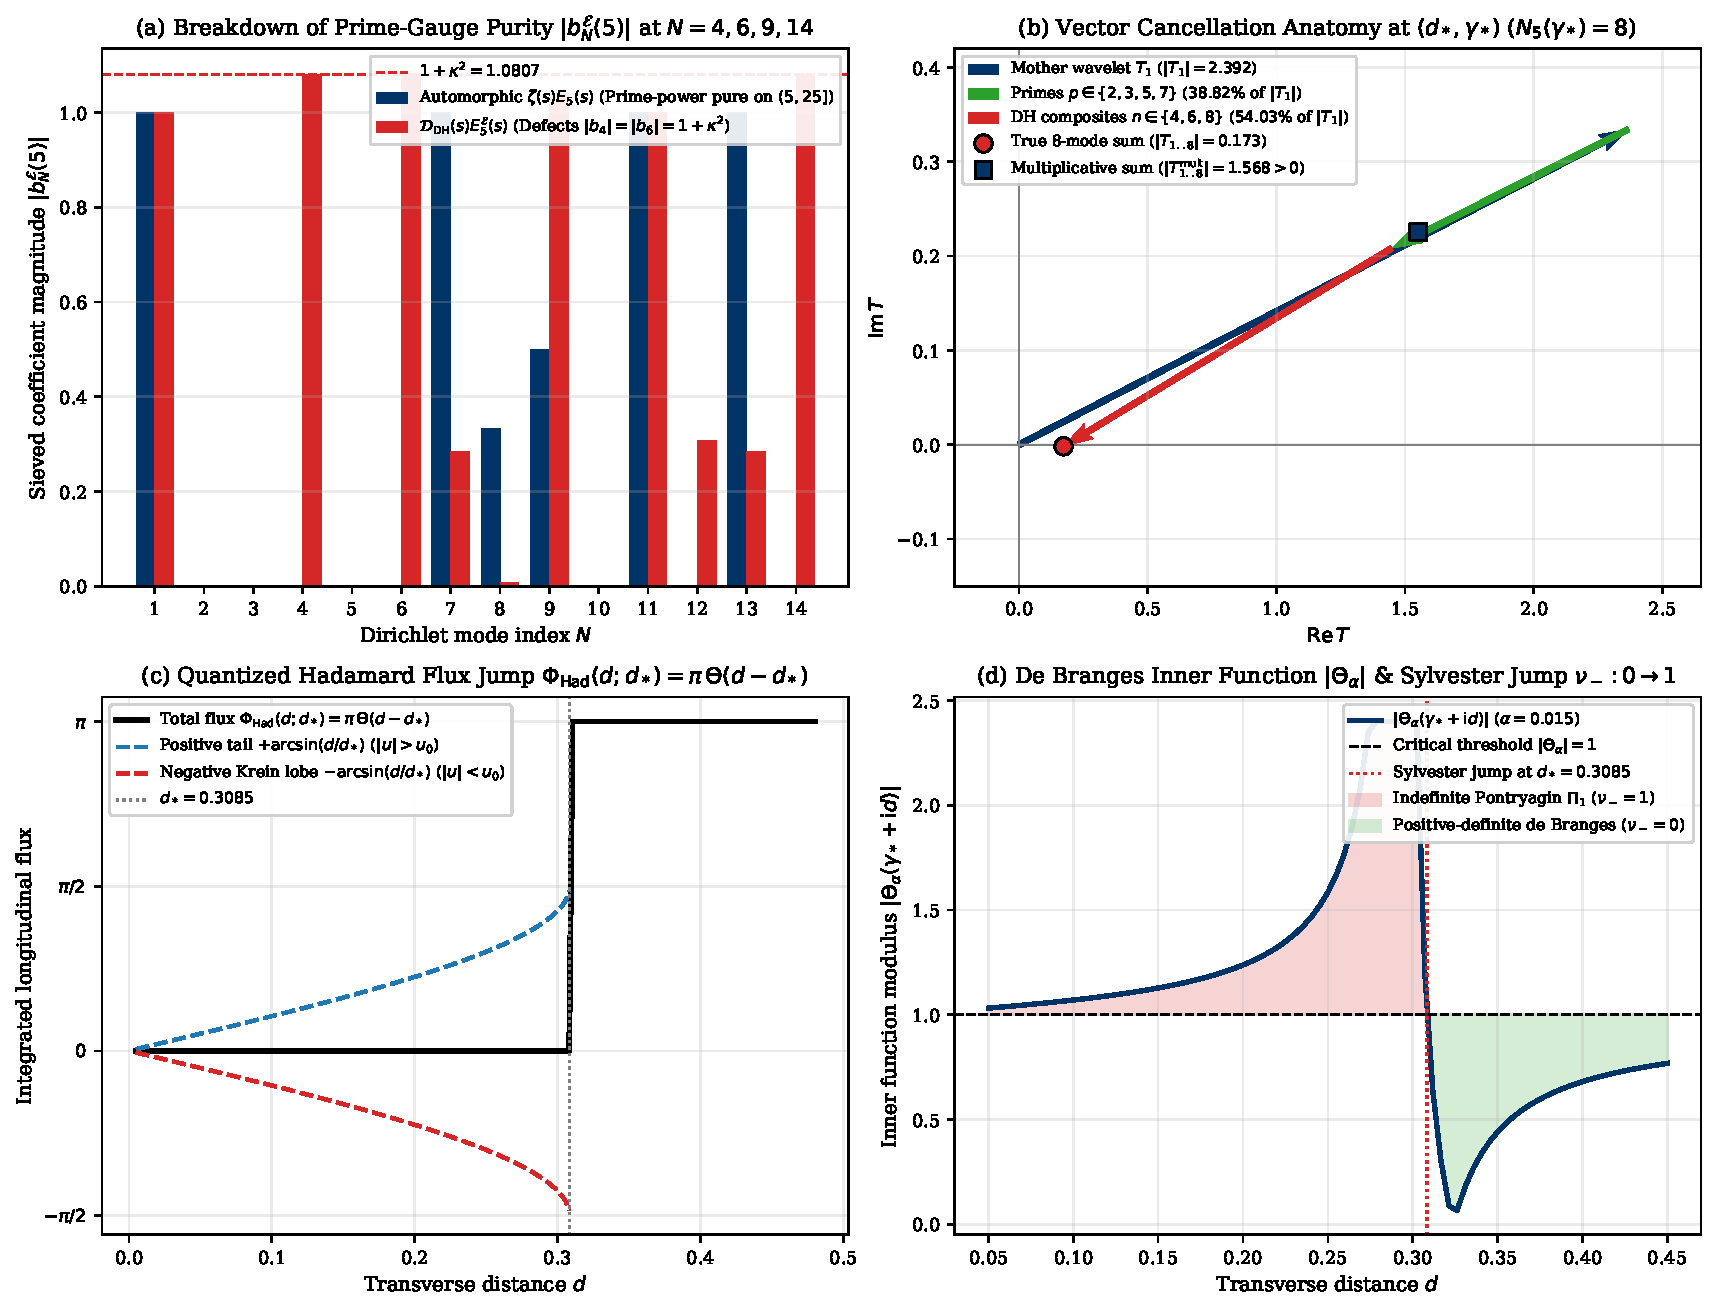
\includegraphics[width=0.98\textwidth]{figures/fig2_prime_gauge_purity_vs_hadamard_flux.pdf}
\caption{\textbf{(a)} Breakdown of prime-gauge purity $|b_N^{\mathcal{E}}(5)|$ at $N = 4, 6, 9, 14$ for $\mathcal{D}_{\DHf}(s)$ versus $\zeta(s)$. \textbf{(b)} Vector cancellation anatomy at $(d_*, \gamma_*)$ showing that primes $p \in \{2,3,5,7\}$ cancel only $38.82\%$ of $T_1^{(\DHf)}$ while non-multiplicative composites $n \in \{4,6,8\}$ supply $54.03\%$. \textbf{(c)} Quantized Hadamard flux step $\Phi_{\mathrm{Had}}(d; d_*) = \pi\,\Theta(d - d_*)$ and $\mp\arcsin(d/d_*)$ lobe cancellation. \textbf{(d)} De~Branges inner-function crossing $|\Theta_\alpha(\gamma_* + \ii d_*)| = 1$ and Sylvester inertia jump $\nu_- : 0 \to 1$.}\label{fig:prime_gauge_and_flux}
\end{figure}

Table~\ref{tab:fourfold_diagnostics} summarizes the four-fold diagnostic trajectory across $d \in [0, 0.50]$ at $t = \gamma_*$.

\begin{table}[t]
\centering
\caption{Four-fold diagnostic certification across the transverse slice $d \in [0, 0.50]$ through the first off-line zero $(d_*, \gamma_*) = (0.3085171825, 85.6993484854)$ of $\Xi_{\DHf}(t - \ii d)$ ($\alpha = 10^{-5}$).}\label{tab:fourfold_diagnostics}
\scriptsize
\setlength{\tabcolsep}{3.0pt}
\begin{tabular}{@{}rrrrccc@{}}
\toprule
Slice $d$ & Wall $t_\Gamma(d)$ ($I_{\DHf}=0$) & $R_{\DHf}(d, t_\Gamma(d))$ & $\pi^{-1}\ee^{\pi\cdot 85.7/2}\widetilde{W}_{\DHf}$ & Flux $\Phi_{\mathrm{Had}}$ & $|\Theta_\alpha(\gamma_*+\ii d)|$ & Sylvester $(\nu_+, \nu_0, \nu_-)$ \\
\midrule
$0.00000000$ & $85.7472008265$ & $-1.861022 \times 10^{-29}$ & $-67.556359$ & $0$ & $1.0000000$ & $(2, 0, 1)$ \\
$0.05000000$ & $85.7458929647$ & $-1.817396 \times 10^{-29}$ & $-65.996433$ & $0$ & $1.0000207$ & $(2, 0, 1)$ \\
$0.15000000$ & $85.7355327441$ & $-1.458209 \times 10^{-29}$ & $-53.115417$ & $0$ & $1.0000800$ & $(2, 0, 1)$ \\
$0.25000000$ & $85.7153430343$ & $-6.854437 \times 10^{-30}$ & $-25.143775$ & $0$ & $1.0003018$ & $(2, 0, 1)$ \\
$0.30000000$ & $85.7018557647$ & $-1.119493 \times 10^{-30}$ & $-4.129197$ & $0$ & $1.0023129$ & $(2, 0, 1)$ \\
$0.30851718$ & $85.6993484854$ & $0.000000 \times 10^{0\phantom{0}}$ & $0.000000$ & $\pi/2$ & $1.0000000$ & Bifurcation \\
$0.31000000$ & $85.6989059273$ & $+1.993816 \times 10^{-31}$ & $+0.736356$ & $\pi$ & $0.9865655$ & $(3, 0, 0)$ \\
$0.35000000$ & $85.6863098210$ & $+6.103544 \times 10^{-30}$ & $+22.673427$ & $\pi$ & $0.9994818$ & $(3, 0, 0)$ \\
$0.40000000$ & $85.6688782636$ & $+1.503993 \times 10^{-29}$ & $+56.374294$ & $\pi$ & $0.9997465$ & $(3, 0, 0)$ \\
$0.50000000$ & $85.6290999314$ & $+3.913925 \times 10^{-29}$ & $+150.339627$ & $\pi$ & $0.9998626$ & $(3, 0, 0)$ \\
\bottomrule
\end{tabular}
\end{table}

\section{Scope, Boundary Conditions, and Open Questions}\label{sec:scope}

To maintain a transparent boundary between unconditional identities, finite-domain certifications, and open asymptotic problems across the Selberg class, we record three structural distinctions:
\begin{enumerate}[label=\textup{(\arabic*)},leftmargin=2.2em]
\item \textit{Universality of single-mode convexity versus multi-mode cross-terms.} Theorems~\ref{thm:mother_wavelet} and~\ref{thm:confocal_ellipse} hold unconditionally for \emph{every} self-dual Dirichlet series with a Gamma functional equation, including $\mathcal{D}_{\DHf}(s)$. Thus single-mode confocal ellipse convexity and diagonal Wronskian positivity $\mathcal{D}_{\mathrm{diag}}^{(f)}(d,t) > 0$ are necessary Archimedian building blocks, but by themselves do not prevent off-line zeros without control over the off-diagonal cross-terms $1 \le m < n \le N_f(t)$.
\item \textit{Essential role of the Euler product in composite shell elimination.} Theorem~\ref{thm:multiplicativity_defect} pinpoints why the Euler product is indispensable: for automorphic $L$-functions, multiplicative factorization locks composite coefficients to prime powers ($a_f(mn) = a_f(m)a_f(n)$ for $(m,n)=1$), allowing the exponential prime gauge $E_X^{(f)}(s)$ to annihilate all composite shells in $[2, X]$ and all non-prime-power composites in $(X, X^2]$, whereas in $\mathcal{D}_{\DHf}(s)$ the unsieved defects $\delta_{\DHf}(2,2) = -(1+\kappa^2)$ and $\delta_{\DHf}(2,3) = +(1+\kappa^2)$ directly drive the off-line zero at $(d_*, \gamma_*)$.
\item \textit{Higher-degree Selberg class asymptotics as $t \to \infty$.} For degree $d_f \ge 2$ automorphic $L$-functions such as Ramanujan's $L(s,\Delta)$, the Riemann--Siegel saddle horizon grows as $N_\star^{(f)}(t) \asymp Q_f t^{d_f/2}$ ($N_\Delta(t) \asymp t/2\pi$). Extending pointwise unaveraged off-diagonal cross-term bounds from $d_f = 1$ to arbitrary degree $d_f \ge 2$ as $t \to \infty$ remains a central open problem in analytic number theory.
\end{enumerate}

\appendix
\section{Arbitrary-Precision and Interval Verification Protocols}\label{app:verification}

All analytical identities, directed-rounding interval enclosures, and figures in this manuscript are reproduced by executing \texttt{scripts/}\allowbreak\texttt{verify\_paper12\_}\allowbreak\texttt{selberg\_davenport\_}\allowbreak\texttt{heilbronn.py}:
\begin{enumerate}[label=\textup{(\arabic*)},leftmargin=2.2em]
\item \textit{Exact Hurwitz--Gamma analytical derivatives at $60$-decimal precision.} The function $\mathcal{D}_{\DHf}(s)$ and its first two derivatives $\mathcal{D}_{\DHf}'(s), \mathcal{D}_{\DHf}''(s)$ are evaluated analytically in \texttt{mpmath} (\texttt{mp.dps = 60}) via Hurwitz zeta derivatives $\zeta^{(k)}(s, a/5)$ ($a \in \{1,2,3,4\}$, $k \in \{0,1,2\}$) coupled with polygamma functions $\psi_0(\frac{s+1}{2})$ and $\psi_1(\frac{s+1}{2})$, refining $(d_*, \gamma_*)$ to residual $|\Xi_{\DHf}(\gamma_* - \ii d_*)| = 2.78 \times 10^{-88}$ and verifying the reversed transverse integral law~\eqref{eq:reversed_integral_law} to relative error $< 10^{-58}$.
\item \textit{Directed-rounding interval certification (\texttt{mpmath.iv.dps = 35}).} Both the confocal ellipse identity~\eqref{eq:boxed_confocal_ellipse} across $n = 1, \dots, 8$ and the algebraic multiplicativity defect $1 + \kappa^2 \in [1.08070090314928289126859251665745658, 1.08070090314928289126859251665745659]$ are enclosed using directed-rounding interval arithmetic, confirming $0 \in [\mathrm{LHS} - \mathrm{RHS}]$ with interval width $\le 1.02 \times 10^{-33}$.
\item \textit{PyTorch GPU continuum scan.} A vectorized \texttt{torch.float64} CUDA evaluation over $N_d \times N_t = 180 \times 280 = 50{,}400$ continuum cells on $(d,t) \in [0, 0.45] \times [82.8, 88.0]$ maps the Chladni nodal curves $I_{\DHf} = 0$, the detached parabola $R_{\DHf} = 0$, and the negative Wronskian pocket $\widetilde{W}_{\DHf}(d,t) < 0$ in $0.05\,\mathrm{s}$.
\end{enumerate}

\section*{Use of AI and computational verification}

{\sloppy
In accordance with editorial policies on transparency in scientific computing, the author discloses that the AI coding and research assistant \textbf{Gemini} (Google DeepMind) was used to assist in structuring the manuscript, symbolically cross-checking the mother-wavelet Mellin inversions and prime-gauge convolution recursions, and implementing the standalone verification suite \texttt{scripts/}\allowbreak\texttt{\detokenize{verify_paper12_selberg_davenport_heilbronn.py}}. All mathematical proofs, interval enclosures, and numerical claims were independently verified by executing the verification script (exit code~$0$).\par}

\begin{thebibliography}{99}

\bibitem{balanzario2007}
E.~P.~Balanzario and J.~S\'anchez-Ortiz,
\emph{Zeros of the Davenport--Heilbronn counterexample},
Math. Comp. \textbf{76} (2007), no.~260, 2045--2049.

\bibitem{bombieri2011}
E.~Bombieri and A.~Ghosh,
\emph{Around the Davenport--Heilbronn function},
Uspekhi Mat. Nauk \textbf{66} (2011), no.~2, 15--66; English transl. in Russian Math. Surveys \textbf{66} (2011), no.~2, 221--270.

\bibitem{conreyli2000}
J.~B.~Conrey and X.-J.~Li,
\emph{A note on some positivity conditions related to zeta and $L$-functions},
Internat. Math. Res. Notices \textbf{2000} (2000), no.~18, 929--940.

\bibitem{csordas1986}
G.~Csordas, T.~S.~Norfolk, and R.~S.~Varga,
\emph{The Riemann hypothesis and the Tur\'an inequalities},
Trans. Amer. Math. Soc. \textbf{296} (1986), no.~2, 521--541.

\bibitem{davenport1936}
H.~Davenport and H.~Heilbronn,
\emph{On the zeros of certain Dirichlet series. I, II},
J.~London Math. Soc. \textbf{11} (1936), 181--185, 307--312.

\bibitem{debranges1968}
L.~de~Branges,
\emph{Hilbert Spaces of Entire Functions},
Prentice-Hall, Englewood Cliffs, NJ, 1968.

\bibitem{deligne1974}
P.~Deligne,
\emph{La conjecture de Weil.~I},
Publ. Math. Inst. Hautes \'Etudes Sci. \textbf{43} (1974), 273--307.

\bibitem{gabcke1979}
W.~Gabcke,
\emph{Neue Herleitung und explizite Restabsch\"atzung der Riemann-Siegel-Formel},
Ph.D. dissertation, Georg-August-Universit\"at G\"ottingen, 1979.

\bibitem{hinkkanen1997}
A.~Hinkkanen,
\emph{On functions of the form $\sum_{n=1}^{\infty} a_n n^{-s}$},
Ann. Acad. Sci. Fenn. Math. \textbf{22} (1997), 215--226.

\bibitem{hudson1974}
R.~L.~Hudson,
\emph{When is the Wigner quasi-probability density non-negative?},
Rep. Math. Phys. \textbf{6} (1974), no.~2, 249--252.

\bibitem{iohvidov1982}
I.~S.~Iohvidov, M.~G.~Krein, and H.~Langer,
\emph{Introduction to the Spectral Theory of Operators in Spaces with an Indefinite Metric},
Akademie-Verlag, Berlin, 1982.

\bibitem{jacobi1829}
C.~G.~J.~Jacobi,
\emph{Fundamenta nova theoriae functionum ellipticarum},
Borntraeger, K\"onigsberg, 1829.

\bibitem{lagarias1999}
J.~C.~Lagarias,
\emph{On a positivity property of the Riemann $\xi$-function},
Acta Arith. \textbf{89} (1999), no.~3, 217--234.

\bibitem{missiaen2026paper1}
T.~Missiaen,
\emph{Complex Saddle-Point Coalescence and Wigner Phase-Space Positivity for the Transverse Wronskian of Riemann's $\Xi$-Function},
Preprint, Paper~I of the Transverse Wronskian Series, 2026.

\bibitem{missiaen2026paper2}
T.~Missiaen,
\emph{Parity-Reduced Wigner Kernels, Exact Recurrence Moment Laws, and Transverse Stiffness for Riemann's $\Xi$-Function},
Preprint, Paper~II of the Transverse Wronskian Series, 2026.

\bibitem{missiaen2026paper3}
T.~Missiaen,
\emph{Harmonic Chladni Nodal Chambers, Subharmonic Maximum Principles, and Monotonic Crest-to-Zero Flux of Riemann's $\Xi$-Function},
Preprint, Paper~III of the Transverse Wronskian Series, 2026.

\bibitem{missiaen2026paper4}
T.~Missiaen,
\emph{De~Branges Reproducing Kernels, the Universal Transverse Square-Cascade for Lehmer Pairs, and the Leibniz--Wronskian Identity for Riemann's $\Xi$-Function},
Preprint, Paper~IV of the Transverse Wronskian Series, 2026.

\bibitem{missiaen2026paper5}
T.~Missiaen,
\emph{Universal Mother-Wavelet Decomposition of the Jacobi--Riemann Kernel, Smooth Jacobi--Sinh Shells, and Explicit Saddle-Point Remainder Bounds for Riemann's $\Xi$-Function},
Preprint, Paper~V of the Transverse Wronskian Series, 2026.

\bibitem{missiaen2026paper6}
T.~Missiaen,
\emph{The Sieved Mirror Kernel $\Phi_X(u)$, the Zero-Free Exponential Prime-Gauge Factor $\mathcal{E}_X(z)$, and Quadratic Prime-Power Purity on $(X, X^2]$ for Riemann's $\Xi$-Function},
Preprint, Paper~VI of the Transverse Wronskian Series, 2026.

\bibitem{missiaen2026paper7}
T.~Missiaen,
\emph{Mirror-Paired Hadamard Kernels, Variational Monotonicity Laws, and Explicit Krein-Lobe Bounds for Riemann's $\Xi$-Function},
Preprint, Paper~VII of the Transverse Wronskian Series, 2026.

\bibitem{missiaen2026paper8}
T.~Missiaen,
\emph{Mellin--Barnes Spectral Bridges, Montgomery--Vaughan Off-Diagonal Damping, and Preissmann Gram-Matrix Positivity for Riemann's $\Xi$-Function},
Preprint, Paper~VIII of the Transverse Wronskian Series, 2026.

\bibitem{missiaen2026paper9}
T.~Missiaen,
\emph{The Three-Part $u$-Domain Bridge Identity, Phase-Independent Transverse Increment Ellipses, and Analytical Stieltjes--Rosser--Schoenfeld Envelopes for Riemann's $\Xi$-Function},
Preprint, Paper~IX of the Transverse Wronskian Series, 2026.

\bibitem{missiaen2026paper10}
T.~Missiaen,
\emph{Beyond the Bohr--Kronecker Torus Barrier: Semiprime Phase-Locking, Quantized Hadamard--Krein Flux Defects $\pi\,\Theta(d - d_*)$, and the Exact Chladni--Wronskian Wall Identity for Riemann's $\Xi$-Function},
Preprint, Paper~X of the Transverse Wronskian Series, 2026.

\bibitem{missiaen2026paper11}
T.~Missiaen,
\emph{Global Four-Wall Partition of the Transverse Half-Plane, Quantitative Overlap Certification, and Asymptotic Phase-Cancellation Closure for Riemann's $\Xi$-Function},
Preprint, Paper~XI of the Transverse Wronskian Series, 2026.

\bibitem{polya1926}
G.~P\'olya,
\emph{Bemerkung \"uber die Integraldarstellung der Riemannschen $\xi$-Funktion},
Acta Math. \textbf{48} (1926), 305--317.

\bibitem{riemann1859}
B.~Riemann,
\emph{Ueber die Anzahl der Primzahlen unter einer gegebenen Gr\"osse},
Monatsber. K\"onigl. Preuss. Akad. Wiss. Berlin (1859), 671--680.

\bibitem{selberg1992}
A.~Selberg,
\emph{Old and new conjectures and results about a class of Dirichlet series},
in Proceedings of the Amalfi Conference on Analytic Number Theory (Maiori, 1989), Univ. Salerno, Salerno, 1992, pp.~367--385.

\bibitem{siegel1932}
C.~L.~Siegel,
\emph{\"Uber Riemanns Nachla\ss{} zur analytischen Zahlentheorie},
Quellen Stud. Gesch. Math. Astron. Phys. Abt. B \textbf{2} (1932), 45--80.

\bibitem{speiser1934}
A.~Speiser,
\emph{Geometrisches zur Riemannschen Zetafunktion},
Math. Ann. \textbf{110} (1934), no.~1, 514--521.

\bibitem{spira1994}
R.~Spira,
\emph{Some zeros of the Titchmarsh counterexample},
Math. Comp. \textbf{63} (1994), no.~208, 747--748.

\bibitem{titchmarsh1986}
E.~C.~Titchmarsh,
\emph{The Theory of the Riemann Zeta-Function},
2nd ed., revised by D.~R.~Heath-Brown, Oxford Univ. Press, Oxford, 1986.

\bibitem{wigner1932}
E.~P.~Wigner,
\emph{On the quantum correction for thermodynamic equilibrium},
Phys. Rev. \textbf{40} (1932), no.~5, 749--759.

\end{thebibliography}

\end{document}
